\documentclass{article}

\usepackage{mathptmx}
%packages for language
\usepackage[czech]{babel}
\usepackage[utf8]{inputenc}
%packages for graphic
\usepackage{graphicx}
\usepackage{pgfplots}
\usepackage{pgfplotstable}
\usepackage{multirow}
\usepackage{tikz}
\usepackage{import}
\usepackage[a4paper, total={17cm,25.7cm}, top=2cm, left=2cm, includefoot]{geometry}
\usepackage{todonotes}
\usepackage{standalone}
\usepackage{colortbl}%pro barevne zmeny v tabulce
\usepackage{float}
\usepackage{csvsimple} %pro import a práci s csv soubory
\usepackage{indentfirst}  % odsazení prvního řádku v odstavci
\usepackage{hyperref} %dela odkazy na mista v dokumentu atd
\usepackage{amsmath}%psani matic
\usepackage{mathrsfs}%psani kroucenym matematickym pismem
\usepackage{pdfpages}%vkladani celych pdf dokumentu

\begin{document}
	
	\documentclass[12pt]{article}
\usepackage{graphicx}
\begin{document}
\begin{titlepage}
\begin{center}
        \huge
        Západočeská Univerzita v Plzni\\
        Fakulta Aplikovaných Věd\\
        
        \vspace{1cm}
        
        \includegraphics[width=0.5\textwidth]{./Graphics/FAV_logo.pdf}
        
        \vspace{4cm}
        \huge
        \textbf{Sytém dvou spojených nádrží}
        
        \vspace{0.5cm}
        \LARGE
        Filip Jašek a Andrea Kadlecová
        
    \end{center} 
    \vfill
        \noindent
        \large
        Předmět: LS1\\
        Přednášející: Ing. Martin Goubej Ph.D.\\
        Cvičící: Ing Martin Čech Ph.D.
\end{titlepage}
\end{document}
	\newpage
	\tableofcontents % generuje obsah
	\newpage
	%\section{Zadání}
		\includepdf[pages={1,2}]{./Graphics/ls1.pdf}
		\newpage
	\section{První část zadání}
		\subsection{Výpočet přepouštěcího a výtokového ventilu}
			Přítoky do první a druhé nádoby jsou definovány vztahy 
			\begin{center}
			$Q_p (t)=c_pS_pv_p(t)$  
			
			\bigskip
			
			$Q_2(t)=c_2S_2v_2(t)$
			\end{center}
			
			Z Bernoulliho rovnice pro průtokový ventil si vyjádříme $v_p$.
			
			\begin{center}
			$p_0+\rho gH_1(t)=p_0+\rho gH_2(t)+\frac{\rho v^2_p(t)}{2}$
			
			$v_p=\sqrt{2g(H_1-H_2)}$ 
			
			\end{center}
			
			Po dosazení za $g=10 \hspace{2mm} m\cdot s^{-2}$, $H_1=0,6 \hspace{2mm} m$ a $H_2=0,4 \hspace{2mm} m$ vyjde 
			
			\begin{center} 
			$v_p=\sqrt{2\cdot10(0,6-0,4)}=\sqrt{20\cdot0,2}=2 \hspace{2mm} ms^{-2}$ 
			\end{center} 
			Pro výtokový ventil se opět použije Bernoulliho rovnice 
			\begin{center}
			$p_0+\rho gH_2(t)=p_0+\frac{\rho v^2_p(t)}{2}$,
			\end{center}
			 ze které se opět vyjádří $v_2$, což je $v_2=\sqrt{2gH_2}$. Po dosazení vyjde $v_2=2\sqrt{2} \hspace{2mm} m \cdot s^{-2}$
			
			Díky tomu, že známe rychlosti průtoků, tak si můžeme z rovnic pro přítoky vyjádřit $S_p$ a $S_2$. Také známe hodnotu $Q_1$. Jelikož chceme udržet hladiny v rovině, tak $Q_p=Q_2=Q_1=1,5 \cdot 10^{-4} \hspace{2mm} m^3 \cdot s^{-1}$.
			\begin{center}
			$S_p=\frac{Q_p}{c_pv_p}=\frac{1,5 \cdot 10^{-4}}{0,6 \cdot 2}=\frac{1,5}{12000}$
			
			\bigskip
			
			$S_2=\frac{Q_2}{c_2v_2}=\frac{1,5 \cdot 10^{-4}}{0,6 \cdot 2\sqrt{2}}=\frac{1,5}{12000\sqrt{2}}$
			
			\end{center}
						
		\subsection{Určení linearizovaného modelu}
			Systém popíšeme dvěma nelineárními diferenciálními rovnicemi. Dostali jsme je z výše uvedených vztahů v části jedna, kde jsme si vyjádřili rychlosti průtoků a vztahy pro přítoky. 
			
			\begin{center} 
			$Q_p (t)=c_pS_pv_p(t)$  
			
			\bigskip
			
			$Q_2(t)=c_2S_2v_2(t)$
			
			\bigskip
			
			$v_p=\sqrt{2 \cdot 10(0,6-0,4)}=\sqrt{20\cdot0,2}=2 \hspace{2mm} m \cdot s^{-2}$ 
			
			\bigskip
			
			$v_2=\sqrt{2gH_2}=2\sqrt{2} \hspace{2mm} m \cdot s^{-2}$
			\end{center} 
			
			Tyto vztahy jsme dosadili do rovnic, které reprezentují rozdíl přítoku a přepouštěcího ventilu a přepouštěcího ventilu s výtokovým ventilem, které se rovnají derivacím objemů nádob podle času a derivaci hladiny podle času násobenou celkovou plochou nádrže.
			\begin{center} 
			$Q_1(t)-Q_p (t)=\frac{dV_1(t)}{dt}=S\frac{H_1(t)}{dt}$  
			
			\bigskip
			
			$Q_p(t)-Q_2(t)=\frac{dV_2(t)}{dt}=S\frac{H_2(t)}{dt}$  
			\end{center}
			
			Po dosazení za $Q_p(t)$, $Q_1(t)$ a $Q_2(t)$ vyjdou dvě nelineární diferenciální rovnice.
			\begin{center}
			$\frac{dH_1(t)}{dt}=-\frac{c_pS_p\sqrt{2g(H_1(t)-H_2(t)}}{S}+\frac{Q_1(t)}{S}$
			
			\bigskip
			
			$\frac{dH_2(t)}{dt}=\frac{c_pS_p\sqrt{2g(H_1(t)-H_2(t))}}{S}-\frac{c_2S_2\sqrt{2gH_2(t)}}{S}$
			\end{center}
			
			Tyto dvě rovnice musíme linearizovat. Po linearizaci vzniknou tyto dvě rovnice, ze kterých pak uděláme matice \textbf{A}, \textbf{B}, \textbf{C} a \textbf{D} a vytvoříme stavový popis mechanismu. 
			
			\begin{center}
			lineární model
			
			\bigskip
			
			$\frac{d\Delta H_1(t)}{dt}=-\frac{c_pS_p\sqrt{2g}}{2S\sqrt{H_1-H_2}}\Delta H_1(t)+\frac{c_pS_p\sqrt{2g}}{2S\sqrt{H_1-H_2}}\Delta H_2(t)+\frac{\Delta Q_1(t)}{S}$
			
			\bigskip
			
			$\frac{d\Delta H_2(t)}{dt}=\frac{c_pS_p\sqrt{2g}}{2S\sqrt{H_1-H_2}}\Delta H_1(t)-(\frac{c_pS_p\sqrt{2g}}{2S\sqrt{H_1-H_2}}+\frac{c_2S_2\sqrt{2g}}{2S\sqrt{H_2}})\Delta H_2(t)$
			
			\bigskip
			
			$\Delta y(t)=\begin{bmatrix}
			0 && 1
			\end{bmatrix}
			\begin{bmatrix}
				\Delta H_1(t)\\
				\Delta H_2(t)
			\end{bmatrix}$
			
			\bigskip
			
			stavový popis
			
			\bigskip
			
			$\begin{bmatrix}
			\Delta \dot{H_1(t)}\\
			\Delta \dot{H_2(t)}
			\end{bmatrix}=\textbf{A}\begin{bmatrix}
			\Delta H_1(t)\\
			\Delta H_2(t)
			\end{bmatrix}+\textbf{B}\Delta Q_1(t)$
			
			\bigskip
			
			$\Delta y(t)=\textbf{C}\begin{bmatrix}
			\Delta H_1(t)\\
			\Delta H_2(t)
			\end{bmatrix}+\textbf{D}\Delta Q_1(t)$
			
\bigskip			
			
			Vypočítáme jednotlivé matice \textbf{A}, \textbf{B}, \textbf{C} a \textbf{D} pomocí již známých hodnot. 

\bigskip			
			
			$\textbf{A}=\begin{bmatrix}
			-\frac{c_pS_p\sqrt{2g}}{2S\sqrt{H_1-H_2}} && \frac{c_pS_p\sqrt{2g}}{2S\sqrt{H_1-H_2}} \\
			\frac{c_pS_p\sqrt{2g}}{2S\sqrt{H_1-H_2}} && -\left(\frac{c_pS_p\sqrt{2g}}{2S\sqrt{H_1-H_2}}+\frac{c_2S_2\sqrt{2g}}{2S\sqrt{H_2}}\right)
			\end{bmatrix}=\begin{bmatrix}
			-\frac{1,5\sqrt{5}}{50\sqrt{0,2}} && \frac{1,5\sqrt{5}}{50\sqrt{0,2}}\\
			\frac{1,5\sqrt{5}}{50\sqrt{0,2}}&& -\left(\frac{1,5\sqrt{5}}{50\sqrt{0,2}}-\frac{1,5\sqrt{5}}{5\sqrt{0,8}}\right)
			\end{bmatrix}$
			
			\bigskip
			
			$\textbf{B}=\begin{bmatrix}
 			\frac{1}{S}\\
			0
			\end{bmatrix}$
			
			\bigskip
			
			$\textbf{C}=\begin{bmatrix}
			0 && 1
			\end{bmatrix}$
			
			\bigskip
			
			$\textbf{D}=0$
			
			\bigskip
			
			stavový popis
			
			\bigskip
			
			$\begin{bmatrix}
			\Delta \dot{H_1(t)}\\
			\Delta \dot{H_2(t)}
			\end{bmatrix}=\begin{bmatrix}
			-\frac{1,5\sqrt{5}}{50\sqrt{0,2}} && \frac{1,5\sqrt{5}}{50\sqrt{0,2}}\\
			\frac{1,5\sqrt{5}}{50\sqrt{0,2}}&& -\left(\frac{1,5\sqrt{5}}{50\sqrt{0,2}}-\frac{1,5\sqrt{5}}{5\sqrt{0,8}}\right)
			\end{bmatrix}\begin{bmatrix}
			\Delta H_1(t)\\
			\Delta H_2(t)
			\end{bmatrix}+\begin{bmatrix}
			\frac{1}{S}\\
			0
			\end{bmatrix}\Delta Q_1(t)$
			
			\bigskip
			
			$\Delta y(t)=\begin{bmatrix}
			0 && 1
			\end{bmatrix}\begin{bmatrix}
			\Delta H_1(t)\\
			\Delta H_2(t)
			\end{bmatrix}$
			\end{center} 
			
			Následně je zadáno, že se má vytvořit lineární model, pokud se přítok zvýší o 20\%. Zvolili jsme, že hladiny nádrží zůstanou stejné a změní se obsah průtokového a výtokového ventilu. Zvýšený průtok je roven $Q=1,5 \cdot 120 \cdot 10^{-6} \hspace{2mm} m \cdot s^{-1}$. 
			
			Jak jsme psali výše, zvolili jsme, že výška hladin zůstane stejná a vypočítáme nové hodnoty pro průtokový a výtokový ventil. Použijeme již vypočítané rychlosti ventilů. $v_p=2 \hspace{2mm} m \cdot s^{-1}$ a $v_2=2\sqrt{2} \hspace{2mm} m \cdot s^{-1}$
			
			\begin{center} 
			
			$S_p=\frac{Q(t)}{c_v p(t)}=\frac{Q}{c_p\sqrt{2g(H_1-H_2)}}=\frac{1,5\cdot 10^{-6}}{0,6 \cdot 2}=\frac{1,5 \cdot 120 \cdot 10^{-6}}{1,2}$
			
			\bigskip

			$S_2=\frac{Q(t)}{c_2v_2(t)}=\frac{Q}{c_2\sqrt{2gH_2}}=\frac{1,5 \cdot 120 \cdot 10^{-6}}{0,6 \cdot 2\sqrt{2}}=\frac{1,5 \cdot 120 \cdot 10^{-6}}{1,2\sqrt{2}}$
			\end{center}
			
			Vypočtené hodnoty obsahů dosadíme do linearizovaného modelu a vypočteme matice \textbf{A}, \textbf{B}, \textbf{C} a \textbf{D}. 
			
			\begin{center}
			lineární model
			
			\bigskip
			
			$\frac{d\Delta H_1(t)}{dt}=-\frac{c_pS_p\sqrt{2g}}{2S\sqrt{H_1-H_2}}\Delta H_1(t)+\frac{c_pS_p\sqrt{2g}}{2S\sqrt{H_1-H_2}}\Delta H_2(t)+\frac{\Delta Q_1(t)}{S}$
			
			\bigskip
			
			$\frac{d\Delta H_2(t)}{dt}=\frac{c_pS_p\sqrt{2g}}{2S\sqrt{H_1-H_2}}\Delta H_1(t)-(\frac{c_pS_p\sqrt{2g}}{2S\sqrt{H_1-H_2}}+\frac{c_2S_2\sqrt{2g}}{2S\sqrt{H_2}})\Delta H_2(t)$
			
			\bigskip
			
			$\Delta y(t)=\begin{bmatrix}
			0 && 1
			\end{bmatrix}
			\begin{bmatrix}
			\Delta H_1(t)\\
			\Delta H_2(t)
			\end{bmatrix}$
			
			\bigskip
			
			stavový popis
			
			\bigskip
			
			$\textbf{A}=\begin{bmatrix}
			-\frac{c_pS_p\sqrt{2g}}{2S\sqrt{H_1-H_2}} && \frac{c_pS_p\sqrt{2g}}{2S\sqrt{H_1-H_2}} \\
			\frac{c_pS_p\sqrt{2g}}{2S\sqrt{H_1-H_2}} && -\left(\frac{c_pS_p\sqrt{2g}}{2S\sqrt{H_1-H_2}}+\frac{c_2S_2\sqrt{2g}}{2S\sqrt{H_2}}\right)
			\end{bmatrix}=\begin{bmatrix}
			-0,18 && 0,18\\
			0,18&& -0,27
			\end{bmatrix}$
			
			\bigskip
			
			$\textbf{B}=\begin{bmatrix}
			\frac{1}{S}\\
			0
			\end{bmatrix}$
			
			\bigskip
			
			$\textbf{C}=\begin{bmatrix}
			0 && 1
			\end{bmatrix}$
			
			\bigskip
			
			$\textbf{D}=0$
			
			\bigskip
			
			stavový popis s určenými maticemi \textbf{A}, \textbf{B}, \textbf{C}, \textbf{D}
			
			\bigskip
			
			$\begin{bmatrix}
			\Delta \dot{H_1(t)}\\
			\Delta \dot{H_2(t)}
			\end{bmatrix}=\begin{bmatrix}
			-0,18 && 0,18\\
			0,18&& -0,27
			\end{bmatrix}\begin{bmatrix}
			\Delta H_1(t)\\
			\Delta H_2(t)
			\end{bmatrix}+\begin{bmatrix}
			\frac{1}{S}\\
			0
			\end{bmatrix}\Delta Q_1(t)$
			
			\bigskip
			
			$\Delta y(t)=\begin{bmatrix}
			0 && 1
			\end{bmatrix}\begin{bmatrix}
			\Delta H_1(t)\\
			\Delta H_2(t)
			\end{bmatrix}$
			\end{center} 
		\newpage
		\subsection{Simulace modelů pro různé hodnoty vstupu}
			Simulace provádíme s přítokem \(Q_{1}=1.5\cdot10^{-4}s^{-1}\) a graficky porovnáváme chování jednotlivých systémů.
			\begin{figure}[H]
				\centering
				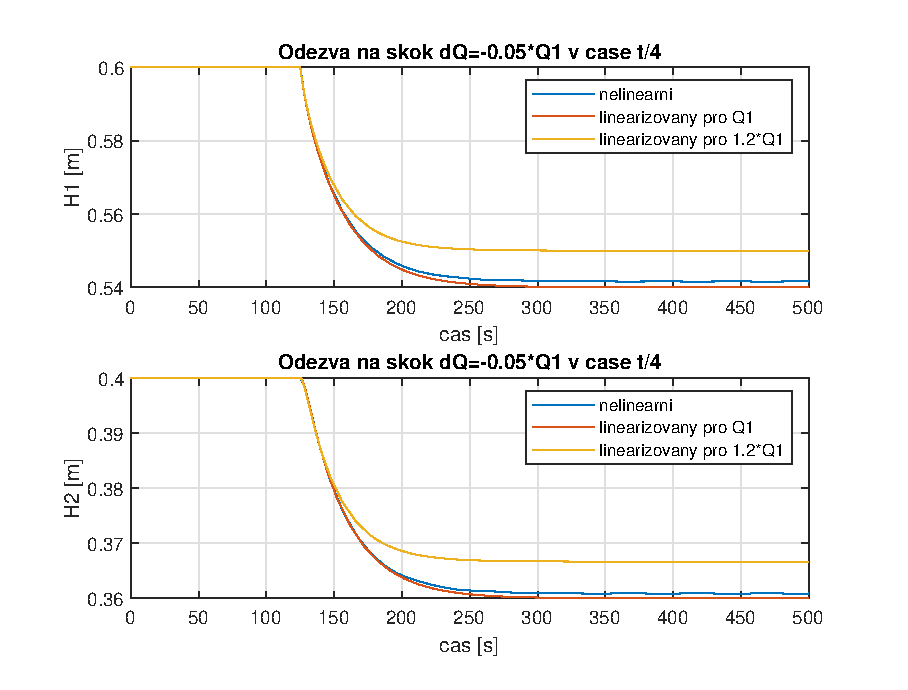
\includegraphics[width=0.85\textwidth]{./Graphics/graphs/C/c_prac_bod_-0.05}\\
				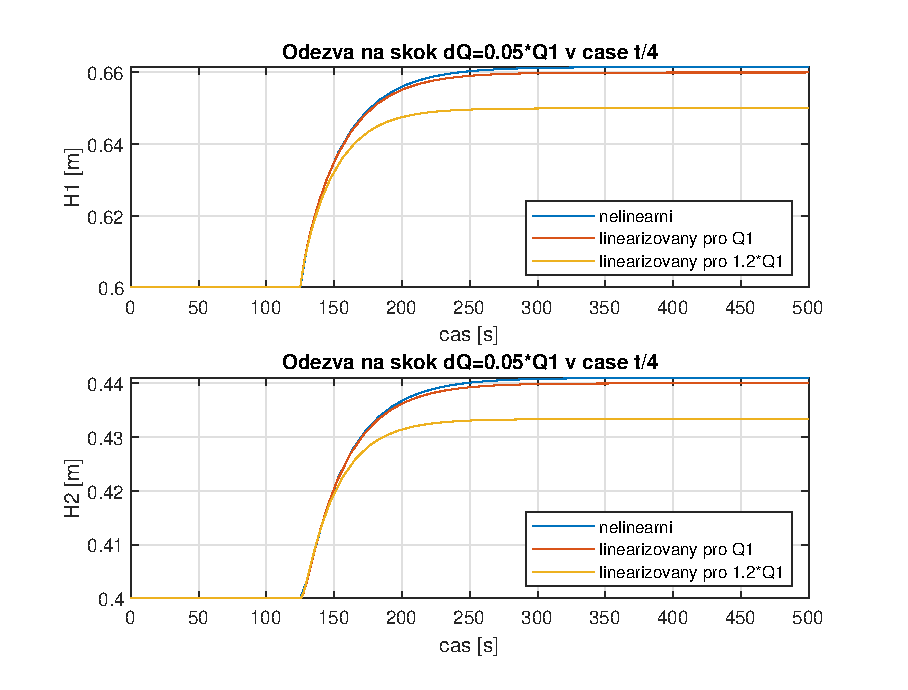
\includegraphics[width=0.85\textwidth]{./Graphics/graphs/C/c_prac_bod_0.05}
				\caption{Chování systémů v okolí pracovního bodu po skokové změně přítoku velikosti dQ jen málo odlišné od \(Q_{1}\).}
				\label{pic:c_prac_bod0.05}
			\end{figure}
			\begin{figure}[H]
				\centering
				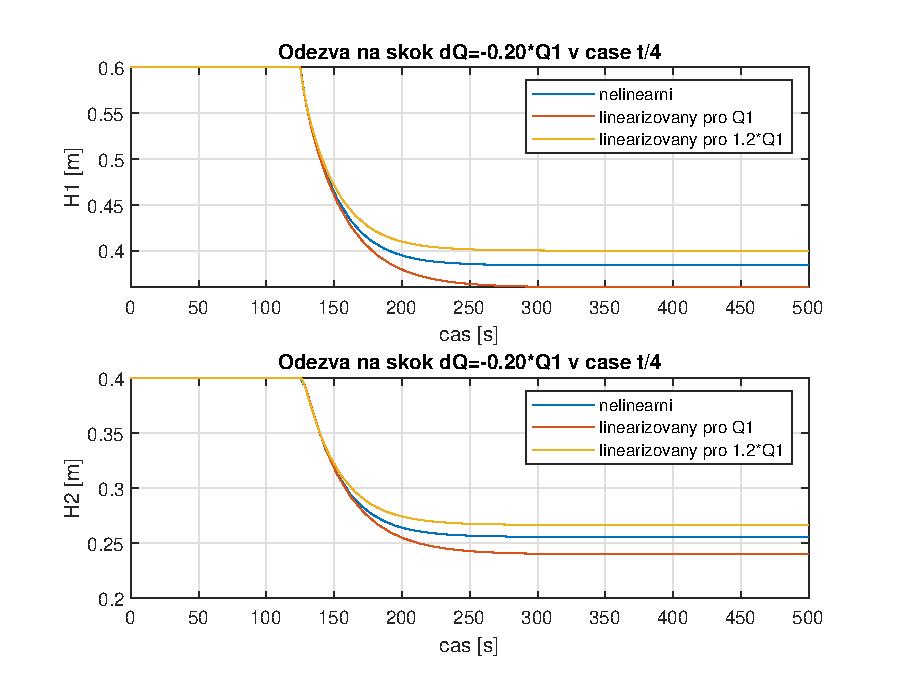
\includegraphics[width=.85\textwidth]{./Graphics/graphs/C/c_prac_bod_-0.20}\\
				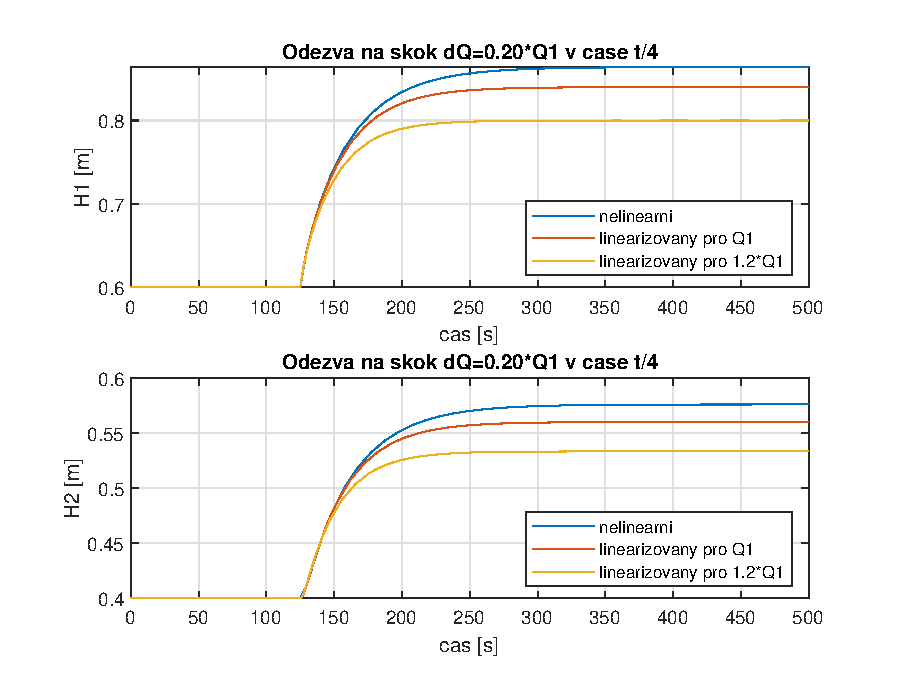
\includegraphics[width=.85\textwidth]{./Graphics/graphs/C/c_prac_bod_0.20}
				\caption{Chování systémů v okolí pracovního bodu po skokové změně přítoku velikosti dQ, kde se přítok zvětší až na hodnotu \(1.2\cdot Q_{1}\).}
				\label{pic:c_prac_bod0.2}
			\end{figure}
			\newpage
			V předchozích grafech můžeme vidět, že pokud se hodnota vstupu skokově odliší jen málo od původního přítoku \(Q_{1}\) (Obrázek \ref*{pic:c_prac_bod0.05}), pak se nelineárnímu modelu blíží více linearizovaný model pro přítok \(Q_{1}\). Když se však skok odliší více, lze pozorovat (Obrázek \ref{pic:c_prac_bod0.2}), že se nelineárnímu modelu začíná více blížit druhý linearizovaný model, který byl spočten pro přítok roven \(1.2\cdot Q_{1}\)
			\begin{figure}[H]
				\centering
				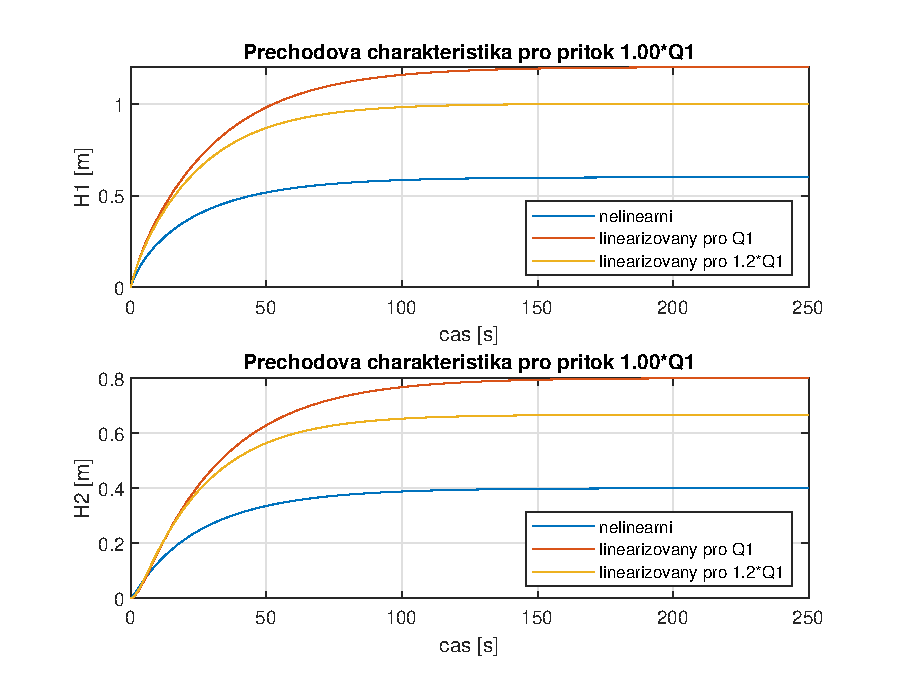
\includegraphics[width=.85\textwidth]{./Graphics/graphs/C/c_100}
				\caption{Přechodové charakteristiky vzniklé působením skokového přítoku o velikosti \(Q_{1}\)}
			\end{figure}
			\begin{figure}[H]
				\centering
				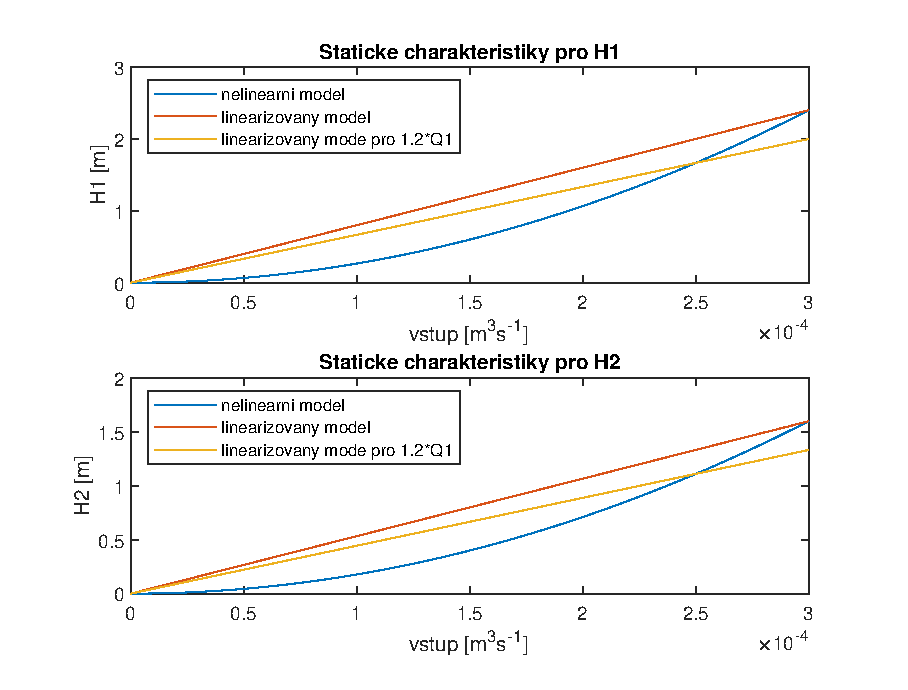
\includegraphics[width=.85\textwidth]{./Graphics/graphs/C/c_stat_char}
				\caption{Statické charakteristiky}
				\label{pic:c_stat_char1}
			\end{figure}
			V z obrázku \ref{pic:c_stat_char1} můžeme vidět, že křivky (přímky) linearizovaných modelů jsou sečnami křivky nelinearního modelu. Posuneme je tedy tak, aby byly tečnou křivky nelineárního modelu. Zde narazíme na problém, že linearizovaný model pro zvýšený průtok se stále odchyluje a jeho tečný bod zcela nesedí s požadovanou ustálenou hodnotou. Děje se to proto, že linearizovaný model je navržen pro přítok \(1.2\cdot Q_{1}\) zatímco v obrázku \ref{pic:c_stat_char1} jsme statickou charakteristiku všech systémů vytvořili pro stejný přítok. Opravu tedy učiníme tak, že při vykreslování statické charakteristiky budeme vstup do systému navrženého pro zvýšený přítok násobit \(1.2\). Tím dostaneme upravenou statickou charakteristiku, kde se statické charakteristiky linearizovaných systémů budou překrývat a tvořit tečnu charakteristiky nelineárního systému přesně v bodě,  pro který jsme nastavili pracovní bod (výšky hladin).
			
			\begin{figure}[H]
				\centering
				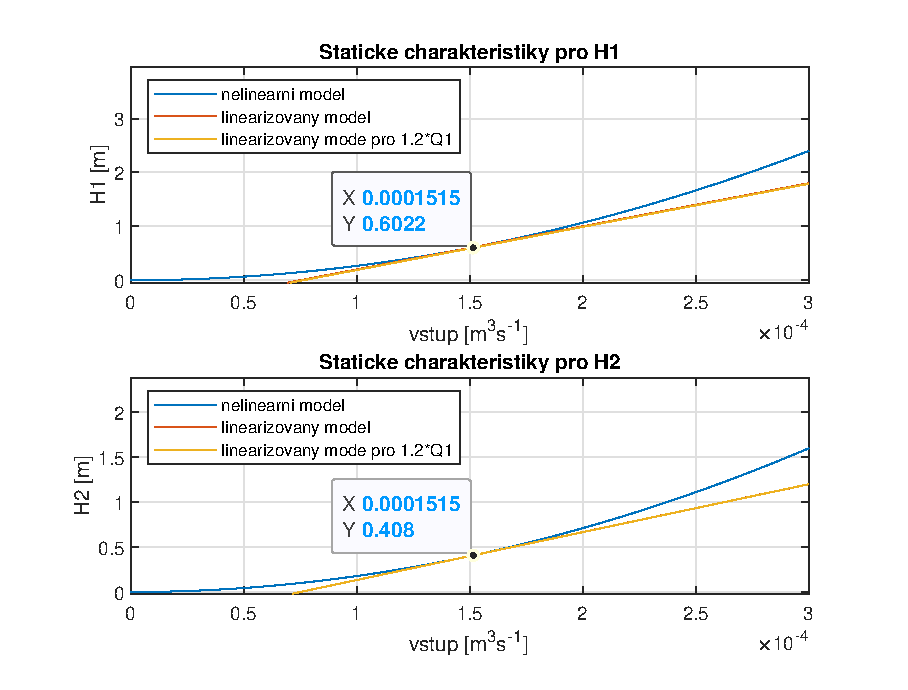
\includegraphics[width=.85\textwidth]{./Graphics/graphs/C/c_stat_char2}
				\caption{Upravené statické charakteristiky, kde linearizované systémy tvoří téměř totožnou tečnu nelineární statické charakteristiky v pracovních bodech nastavených pro jednotlivé hladiny.}
				\label{pic:c_stat_char2}
			\end{figure}
				
			
		\subsection{Určení přenosu}
			Z prvního vypočteného linearizovaného modelu určíme přenosy
				\begin{center}
					$ F_{1}(p)=\frac{Y_{1}(p)}{Q_{1}(p)} $ \hspace{1cm} a \hspace{1cm} $ F_{2}(p)=\frac{Y_{2}(p)}{Q_{1}(p)} $,
				\end{center}
			kde \(Y_{1}(p) = H_{1}(p)\) a \(Y_{2}(p) = H_{2}(p)\). Hledáme tedy přenosovou funkci pro popsání přenosu signálu ze vstupu (přítok \(Q_{1}\)) na výstup, čímž jsou výšky hladin v jednotlivých nádržích.
			Podle příkladu ve skriptech (str. 44) využijeme znalost, že přenos 
			\[F(p)=\textbf{C}(p \textbf{I}-\textbf{A})^{-1}\textbf{B}\]
			a určíme požadované přenosy dosazením za \(\textbf{A}\), \(textbf{B}\) a \(\textbf{C}\). Vektor \(\textbf{C}\) volíme podle toho, který přenos chceme právě zjistit. Pokud přenos \(F_{1}\) pak \(\textbf{C}=\begin{bmatrix}1&&0\end{bmatrix}\) a pokud \(F_{2}\), tak \(\textbf{C}=\begin{bmatrix}0&&1\end{bmatrix}\). Výpočet lze provést i ručně, my však použijeme v programu Matlab jeden řádek kódu \verb|Fp=C*inv(p*eye(2)-A)*B|, který nám vypočte potřebné přenosy.
			
			 Za \(\textbf{C}\) jsme dosadili matici \(\textbf{C}=\begin{bmatrix}1&&0\\0&&1\end{bmatrix}\) čímž nám do proměnné \(Fp\) uloží přímo oba přenosy, kde první se bude vázat k výšce hladiny v první nádobě díky prvnímu řádku matice \(\textbf{C}\) a druhý k výšce hladiny ve druhé nádobě. Z vypočteného přenosu
			\[F_{1}(p)=\frac{400 p + 90}{p^2 + 0,375 p + 0,01125}\]
			určíme nuly přenosu tak, že čitatel položíme roven nule
			\[400p + 90=0\]
			a dopočteme kořeny polynomu, tak aby rovnost platila a označíme je jako nuly přenosu.
			\[z_{1}=-\frac{90}{400}=-0,225\]
			
			Abychom zjistili póly přenosu položíme jmenovatel roven nule
			\[p^2 + 0.375\cdot p + 0.01125=0.\]
			Řešením kvadratické rovnice dostanu její kořeny
			\[p_{1}=\frac{-15+3\cdot\sqrt{17}}{80}\approx -0.0329 \hspace{1cm} p_{2}=\frac{-15-3\cdot\sqrt{17}}{80}\approx -0.3421,\] což jsou zároveň póly přenosu.
			Statické zesílení a časové konstanty budou zřejmé z upraveného tvaru přenosu:
			\[F_{1}(p)=\frac{400p+90}{p^{2}+0.375p+0.01125}=\frac{90\cdot(\frac{400}{90}p+1)}{0.01125(\frac{1}{0.01125}p^{2}+\frac{0.375}{0.01125}p+1)}\]
			Časové konstanty:  \(T_{1}=\sqrt{\frac{1}{0.01125}}=9.428090416\), \(T_{2}=\frac{400}{90}=\frac{40}{9}\)\\
			Statické zesílení: \(K=\frac{90}{0.01125}=8000\)\\
			Pro přenos \[F_{2}(p)=\frac{60}{p^2 + 0.375\cdot p + 0.01125}\] použijeme stejný postup jako u předchozího přenosu a zjistíme, že nulu nemá přenos žádnou a póly jsou totožné. Zesílení zde bude \(K=\frac{60}{0.01125}=5333.\overline{33}\). Časovou konstantu má přenos pouze jednu \(T_{1}=\sqrt{\frac{1}{0.01125}}=\frac{20\sqrt{2}}{3}=9.428090416\)\\\\
			Přenos \(F_{2}(p)\) rozložíme na parciální zlomky, aby se lépe prováděla inverzní Laplaceova transformace, a vyjádříme \(Y_{2}(p)\).
			\[F_{2}(p)=\frac{Y_{2}(p)}{Q_{1}(p)}\hspace{5mm} \rightarrow \hspace{5mm} Y_{2}(p)=Q_{1}(p)\cdot(-\frac{194.0285}{p+0.3421})+Q_{1}(p)\cdot(\frac{194.0285}{p+0.0329})\]
			Nyní vypočtu impulsní funkci tak, že za \(Q_{1}(p)\) dosadím Diracův puls v Laplaceově transformaci, kde má hodnotu \(1\). Provedu inverzní Laplaceovu transformaci a získám tak impulsní funkci v časové oblasti pro přenos \(F_{2}(p)\) jako
			\[y_{2}(t)=194.0285\cdot\left(-e^{-0.3421\cdot t}+e^{-0.0329\cdot t}\right).\]
			Podobně získáme i přechodovou charakteristiku, kde však dosadíme za \(Q_{1}(p)\) Heavisidovu funkci v Laplaceově transformaci, což je \(\frac{1}{p}\). Po inverzní Laplaceově transformaci dostaneme přechodovou funkci ve tvaru
			\[y_{2}(t)=-\frac{194.0285}{0.3421}\cdot(1-e^{-0.3421\cdot t})+\frac{194.0285}{0.0329}\cdot(1-e^{-0.0329\cdot t}).\]
			
			Pro oveření správnosti vypočtených funkcí si je necháme vykreslit spolu s naším dříve odvozeným linearizovaným modelem.
			\begin{figure}[H]
				\centering
				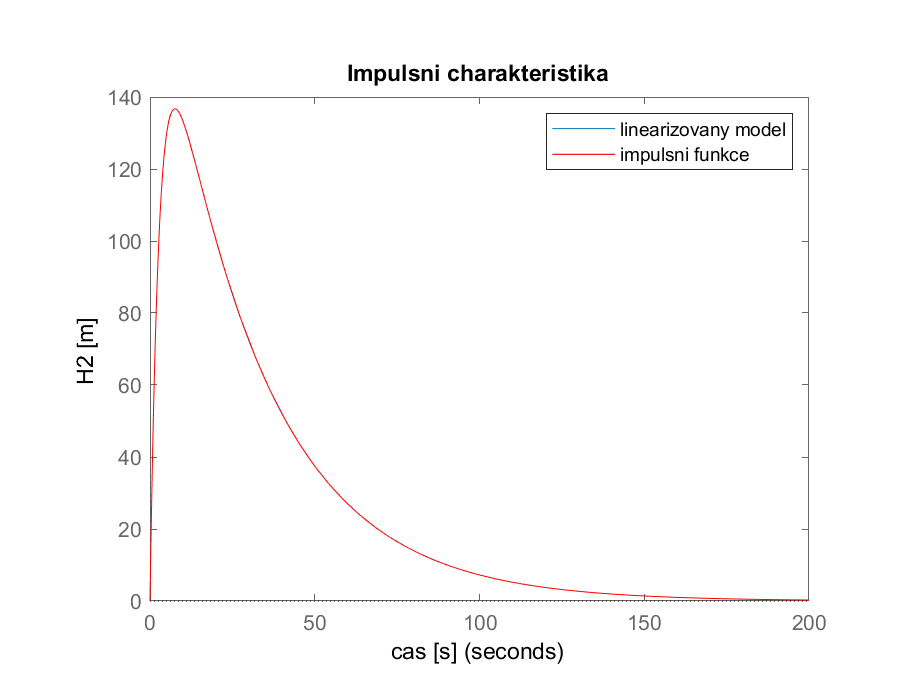
\includegraphics[width=.8\textwidth]{./Graphics/graphs/D/d_imp_char.eps}
				\caption{Graf zobrazující impulsní charakteristiku prvního linearizovaného modelu a vypočtené impulsní funkce}
				\label{graph:d_impulsni_char}			
			\end{figure}
			\begin{figure}[H]
				\centering
				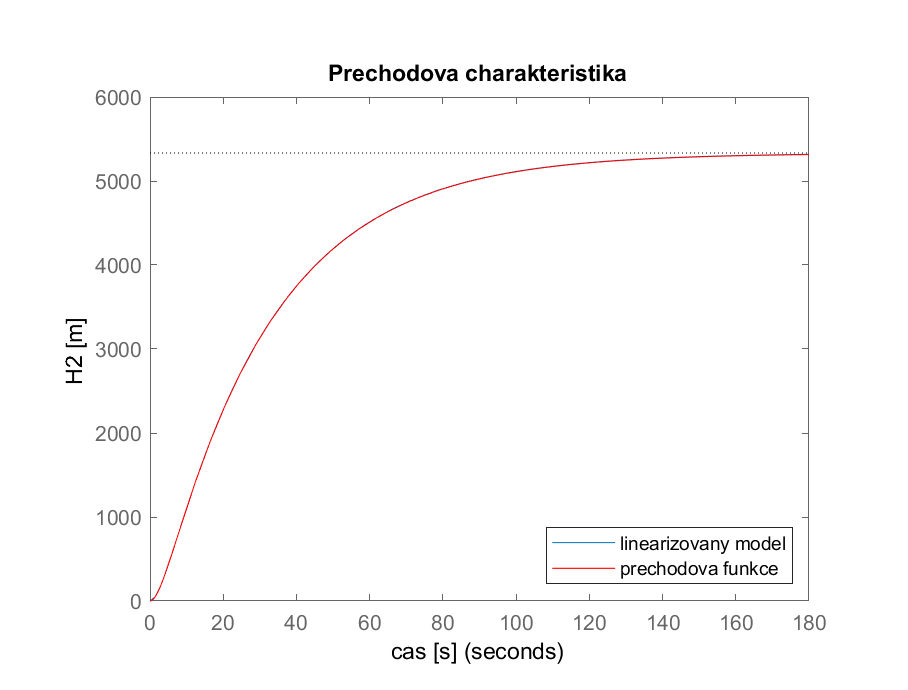
\includegraphics[width=.8\textwidth]{./Graphics/graphs/D/d_prech_char.eps}
				\caption{Graf zobrazující přechodovou charakteristiku prvního linearizovaného modelu a vypočtené přechodové funkce}
				\label{graph:d_prechodova_char}
			\end{figure}
			Na linearizovaný model jsme použili funkci pro přechodovou charakteristiku \verb|step()| a pro impulsní \verb|impulse()|. Z grafů na obrázcích \ref{graph:d_impulsni_char} a \ref{graph:d_prechodova_char} můžeme vidět, že se téměř překrývají a z toho můžeme usoudit, že funkce jsou vypočtené správně, protože se chovají téměř stejně.
		\subsection{Stavová reprezentace}
			Přenos \(F_{2}(p)\) vyjádříme dále pomocí Frobeniovy a Jordanovy stavové reprezentace.\\\\
			\textbf{Frobeniova reprezentace}\\
			Nejprve převedeme přenos na požadovaný tvar
				\[F(p)=K+\frac{b_{1}p+b_{0}}{p^{2}+a_{1}p+a_{0}},\]
			abychom pomocí koeficientů \(K,b_{1},b_{0},a_{1},a_{0}\) mohli sestavit Frobeniovu stavovou reprezentaci ve tvaru
				\[\overline{S}_{frob}:\begin{bmatrix}
					0&1\\
					-a_{0}&-a_{1}
				\end{bmatrix}
				\begin{bmatrix}
					x_{1}(t)\\
					x_{2}(t)
				\end{bmatrix}+
				\begin{bmatrix}
					0\\1
				\end{bmatrix}u(t)\]
				\[y(t)=\begin{bmatrix}
					b_{0}&b_{1}
				\end{bmatrix}
				\begin{bmatrix}
					x_{1}(t)\\
					x_{2}(t)
				\end{bmatrix}+Ku(t).\]
			Z přenosu \(F_{2}(p)=\frac{60}{p^2 + 0,375 p + 0,01125}\) určíme koeficienty 	\(a_{1}=0,375 ,a_{0}=0,01125\), dosadíme je do požadovaného přenosu
				\[[F_{2}(p)=K+\frac{b_{1}p+b_{0}}{p^{2}+0,375p+0,01125},\]
			převedeme na společného jmenovatele
				\[[F_{2}(p)=\frac{Kp^{2}+(0,375K+b_{1})p+(0,01125K+b_{0})}{p^{2}+0,375p+0,01125}\]
			a porovnáním jednotlivých koeficientů s původním přenosem zjistíme koeficienty
				\[K=0\]
				\[0,375K+b_{1}=0 \rightarrow b_{1}=0\]
				\[0,01125K+b_{0}=60 \rightarrow b_{0}=60.\]
			Dosadíme je do Frobeniovy stavové reprezentace a získáme systém ve tvaru
				\[\overline{S}_{frob}:\begin{bmatrix}
					0&1\\
					-0,01125&-0,375
				\end{bmatrix}
				\begin{bmatrix}
					x_{1}(t)\\
					x_{2}(t)
				\end{bmatrix}+
				\begin{bmatrix}
					0\\1
				\end{bmatrix}u(t)\]
				\[y(t)=\begin{bmatrix}
					60&0
				\end{bmatrix}
				\begin{bmatrix}
					x_{1}(t)\\
					x_{2}(t)
				\end{bmatrix}+0u(t).\]
			\textbf{Jordanovu stavovou reprezentaci} vyjádříme ze stavového modelu přenosu \(F_{2}(p)\)
				\[\begin{pmatrix}
					\Delta \dot{H_1(t)}\\
					\Delta \dot{H_2(t)}
				\end{pmatrix}=\begin{pmatrix}
					-0.15 && 0.15\\
					0.15&& -0.225
				\end{pmatrix}\begin{pmatrix}
					\Delta H_1(t)\\
					\Delta H_2(t)
				\end{pmatrix}+\begin{pmatrix}
					400\\
					0
				\end{pmatrix}\Delta Q_1(t)\]
				\[\Delta y(t)=\begin{pmatrix}
					0 && 1
				\end{pmatrix}\begin{pmatrix}
					\Delta H_1(t)\\
					\Delta H_2(t)
				\end{pmatrix}\]
			Ze sbírky příkladů víme, že potřebujeme získat transformační matici \(T_{Jord}\) podle vztahu 
				\[T_{Jord}=V^{-1},\]
			kde \(V\) je matice vlastních vektorů matice \(\textbf{A}\) našeho původního systému.
			Postupujeme tak, že zjistíme vlastní čísla a vlastní vektory matice \(A\) s pomocí příkazu v Matlabu \verb*|eig()|, který nám najde naše vlastní čísla i vektory pomocí zadáním v následujícím tvaru: \verb*|[vlVektory,Aspektralni]=eig(A)|. Do proměnné \verb*|vlVektory| se nám uloží matice vlastních vektorů a do \verb*|Aspektralni| spektrální matice s vlastními čísly na diagonále matice, což je naše nová matice \(\overline{A}_{J}\). Získanou matici vlastních vektorů můžeme zapsat do proměnné \(V\), aby byla zachována analogie s dříve zmíněným vztahem.
			Transformační matici \(T_{J}\) dostaneme pak inverzí matice vlastních vektorů \(V\) a dopočteme matice \(\overline{B}_{J},\overline{C}_{J}\) za pomoci následujících výpočtů:
				\[T_{J}=V^{-1}\]
				\[\overline{A}_{J}=\begin{bmatrix}
					-0,3421&0\\
					0&-0,0329
				\end{bmatrix}\]
				\[\overline{B}_{J} = T_{J}B = \begin{bmatrix}
					-0,6154&0,7882\\
					-0,7882&-0,6154
				\end{bmatrix}\begin{bmatrix}
					400\\0
				\end{bmatrix}=\begin{bmatrix}
					-246,1649\\-315,2822
				\end{bmatrix}\]
				\[\overline{C}_{J}=CT_{J}^{-1}=\begin{bmatrix}
					0&1
				\end{bmatrix}\begin{bmatrix}
					-0,6154&-0,7882\\
					0,7882&-0,6154
				\end{bmatrix}=\begin{bmatrix}
					0,7882&-0,6154
				\end{bmatrix}\]
				\[\overline{D}_{J}=D=0\]
			\vspace{1cm}\\
			V následujících grafech můžeme pozorovat jak všechny tři systémy reagují na Diracův puls a jednotkový skok. Z grafů je patrné, že všechny tři systému jsou z pohledu vstupně-výstupního chování totožné. To jen potvrzuje správnost našeho výpočtu a teorii, že jeden systém lze popsat různými stavovými modely.
				\begin{figure}[H]
					\centering
					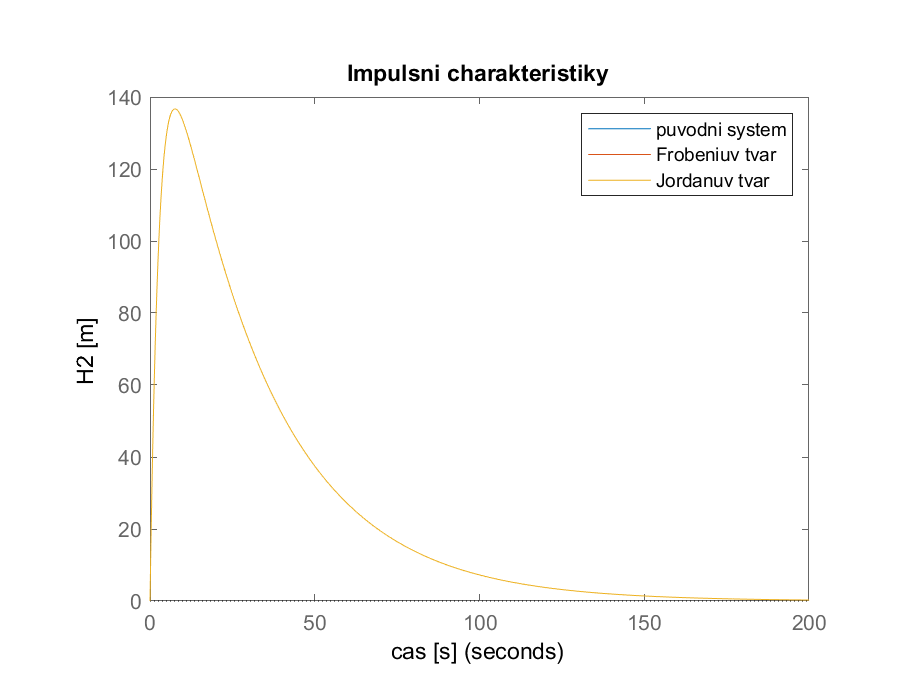
\includegraphics[width=.8\textwidth]{./Graphics/graphs/E/Imp_char_porovnani}
					\caption{Impulsní charakteristiky všech tří systémů.}
				\end{figure}
				\begin{figure}[H]
					\centering
					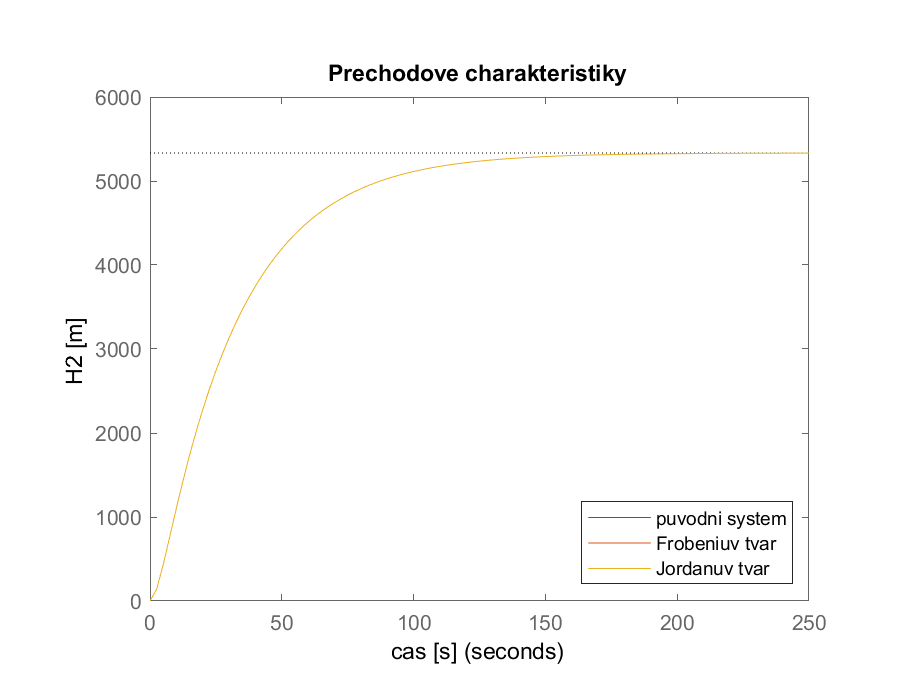
\includegraphics[width=.8\textwidth]{./Graphics/graphs/E/Prech_char_porovnani}
					\caption{Přechodové charakteristiky všech tří systémů.}
				\end{figure}
			\newpage
			\noindent \textbf{Oveření stability}\\
			Začneme zkoumáním vnitřní stability a tedy polohy pólů přenosu původní stavové reprezentace a vlastních čísel matice \(\overline{A}_{Frob}\) a \(\overline{A}_{Jord}\), které zjistíme pomocí příkazu \verb*|eig()| a nebo ručně hledáním kořenů polynomu\(det(\lambda I-A)=0\).\\
			Původní reprezentace přenosem:
			\[F_{2}(p)=\frac{60}{p^2 + 0,375 p + 0,01125}=\frac{60}{(p+0,3421)(p+0,0329)}\]
			Z tvaru jmenovatele je zřejmé, že reálné části pólů leží v záporné polorovině $\Rightarrow$systém je vnitřně stabilní
			Frobeniova stavová reprezentace:
			\[\overline{A}_{Frob}=\begin{bmatrix}
				0&1\\
				-0,01125&-0,375
			\end{bmatrix}\rightarrow \lambda_{1}=-0,0329,\lambda_{2}=-0,3421\]
			Obě vlastní čísla (jejich reálné složky) leží v záporné polorovině $\Rightarrow$ systém je vnitřně stabilní.\\
			Jordanova stavová reprezentace:
			(Zde se vlastní čísla nachází přímo na diagonále matice \(A\))
			\[\overline{A}_{J}=\begin{bmatrix}
				-0,3421&0\\
				0&-0,0329
			\end{bmatrix}\rightarrow \lambda_{1}=-0,3421,\lambda_{2}=-0,0329\]
			Vlastní čísla se opět nachází v záporné polorovině a tedy $\Rightarrow$ systém je vnitřně stabilní.\\
			Jelikož vnitřní stabilita implikuje vnější stabilitu, jsou zmíněné tři reprezentace jak vnitřně stabilní, tak BIBO stabilní.\\\\
			\noindent
			\textbf{Ověření řiditelnosti a pozorovatelnosti}\\
			Řiditelnost a pozorovatelnost systémů ověřím díky porovnání hodností matice \textbf{A} s maticí řiditelnosti a pozorovatelnosti. Pokud má některá matice hodnost jinou než matice \(\textbf{A}\) pak systém nesplňuje podmínky řiditelnosti nebo pozorovatelnosti podle toho, která matice danou podmínku nesplňuje.
			Matici řiditelnosti \(Q_{r}\) vypočítáme jako
				\[Q_{r}=\begin{bmatrix}
					\textbf{B}&\textbf{AB}
				\end{bmatrix}\]
			A matici pozozrovatelnosti \(Q_{p}\) jako
				\[Q_{p}=\begin{bmatrix}
					\textbf{C}\\\textbf{CA}
				\end{bmatrix}\]\\
			Původní stavová reprezentace
				\[Q_{r}=\begin{bmatrix}
					\textbf{B}&\textbf{AB}
				\end{bmatrix}=\begin{bmatrix}
					400&-60\\
					0&60
				\end{bmatrix}\]\hspace{11cm}rank(\(Q_{r}\))=2=n $\Rightarrow$ systém je řiditelný
				\[Q_{p}=\begin{bmatrix}
					\textbf{C}\\\textbf{CA}
				\end{bmatrix}=\begin{bmatrix}
					     0    1,0000
					0,1500   -0,2250
				\end{bmatrix}\]\hspace{11cm}rank(\(Q_{p}\))=2=n $\Rightarrow$ systém je pozorovatelný\\
			Frobeniova reprezentace
				\[Q_{r}=\begin{bmatrix}
					B&AB
				\end{bmatrix}=\begin{bmatrix}
					0&1\\
					1&-0,3750
				\end{bmatrix}\]\hspace{11cm}rank(\(Q_{r}\))=2=n $\Rightarrow$ systém je řiditelný
				\[Q_{p}=\begin{bmatrix}
					\textbf{C}\\ \textbf{CA}
				\end{bmatrix}=\begin{bmatrix}
					60&0\\
					0&60
				\end{bmatrix}\]\hspace{11cm}rank(\(Q_{p}\))=2=n $\Rightarrow$ systém je pozorovatelný\\
			Jordanova reprezentace
				\[Q_{r}=\begin{bmatrix}
					\textbf{B}& \textbf{AB}
				\end{bmatrix}=\begin{bmatrix}
					-246,1649&84,2171\\
					-315,2822&10,3676
				\end{bmatrix}\]\hspace{11cm}rank(\(Q_{r}\))=2=n $\Rightarrow$ systém je řiditelný
				\[Q_{p}=\begin{bmatrix}
					\textbf{C}\\ \textbf{CA}
				\end{bmatrix}=\begin{bmatrix}
					0&1\\
					0,1500&-0,2250
				\end{bmatrix}\]\hspace{11cm}rank(\(Q_{p}\))=2=n $\Rightarrow$ systém je pozorovatelný\\
	\newpage
	\section{Druhá část zadání (advanced models)}
		Nyní v druhé části se budeme věnovat modelu, který rozšíříme o elektrické čerpadlo, které nám bude poskytovat přítok do systému. Ze zadání víme, že je popsáno aperiodickým členem 1. řádu s časovou konstantou \(T=0,5s\) a statickým zesílením \(K_{s}=Q_{1}=1,5\cdot10^{-4} \hspace{2mm} m^{3}\cdot s^{-1}\). Přenos čerpadla od napětí na kotvě motoru k výtoku kapaliny je tedy
		\[F_{cerp}=\frac{Q_{1}}{Tp +1}=\frac{1,5\cdot10^{-4}}{0,5 p+1}\cdot\frac{2}{2}=\frac{3\cdot10^{-4}}{p+2}.\]
		\subsection{Stavový model rozšířené soustavy}
			Aby se dal určit stavový model celé soustavy, potřebujeme z přenosu čerpadla získat diferenciální rovnici pomocí zpětné Laplaceovy transformace následujícím způsobem.
			\[F_{cerp}(p)=\frac{3\cdot10^{-4}}{p+2}\]
			\[\frac{Y(p)}{U(p)}=\frac{3\cdot10^{-4}}{p+2}\]
			\[pY(p) + 2 Y(p)=3\cdot10^{-4} U(p)\hspace{1cm} /\mathscr{L}^{-1}\{\}\]
			\[\dot{y}(t)+2 y(t)=3\cdot10^{-4} u(t)\]
			Jelikož je výstup této diferenciální rovnice (\(y(t)\)) zároveň vstupem do našeho původního linearizovaného systému, přejmenujeme ho na \(q(t)\) a vstup diferenciální rovnice (\(u(t)\)) na \(U_{K}(t)\) (napětí na kotvě motoru čerpadla). Pro lepší názornost  přepíšeme do původních diferenciálních rovnic.
			
			\[\frac{d\Delta H_1(t)}{dt}=-\frac{c_pS_p\sqrt{2g}}{2S\sqrt{H_1-H_2}}\Delta H_1(t)+\frac{c_pS_p\sqrt{2g}}{2S\sqrt{H_1-H_2}}\Delta H_2(t)+\frac{\Delta q(t)}{S}\]
			
			\[\frac{d\Delta H_2(t)}{dt}=\frac{c_pS_p\sqrt{2g}}{2S\sqrt{H_1-H_2}}\Delta H_1(t)-(\frac{c_pS_p\sqrt{2g}}{2S\sqrt{H_1-H_2}}+\frac{c_2S_2\sqrt{2g}}{2S\sqrt{H_2}})\Delta H_2(t)\]
			
			\[\frac{d\Delta q(t)}{dt}=-2\Delta q+3\cdot10^{-4}U_{K}(t)\]
			
			Nyní vypočteme matice lineárního modelu
			\[\textbf{A}=\begin{bmatrix}
				-0,15&0,15&400\\
				0,15&-0,225&0\\
				0&0&-2
			\end{bmatrix}\]
		
			\[\textbf{B}=\begin{bmatrix}
				0\\
				0\\
				3\cdot10^{-4}
			\end{bmatrix}\]
			
			\[\textbf{C}=\begin{bmatrix}
				0&1&0
			\end{bmatrix}\]
		
			\[\textbf{D}=0\]
			
			a dosadíme do stavového popisu
			\[\begin{bmatrix}
				\dot{H_1(t)}\\
				\dot{H_2(t)}\\
				\dot{q(t)}
			\end{bmatrix} = 
			\begin{bmatrix}
				-0,15&0,15&400\\
				0,15&-0,225&0\\
				0&0&-2
			\end{bmatrix}
			\begin{bmatrix}
				H_1(t)\\
				H_2(t)\\
				q(t)
			\end{bmatrix}+
			\begin{bmatrix}
				0\\
				0\\
				3\cdot10^{-4}
			\end{bmatrix} U_{K}(t)\]
		
			\[y(t)=
			\begin{bmatrix}
				0&1&0
			\end{bmatrix}\cdot
			\begin{bmatrix}
				H_1(t)\\
				H_2(t)\\
				q(t)
			\end{bmatrix}\]
		
		Nyní dopočteme přenosové funkce nového linearizovaného systému od napětí na kotvě na jednotlivé výšky hladin pomocí dříve použitého vztahu
		\[F(p)=\textbf{C}(p \textbf{I}-\textbf{A})^{-1}\textbf{B}\]
		jeho zadáním do Matlabu a tvaru matice \[\textbf{C}=\begin{bmatrix}
			1&0&0\\
			0&1&0
		\end{bmatrix}\]
		nám rovnou vrátí naše hledané přenosové funkce
		\[F_{1}(p)=\frac{H_{1}(p)}{U_{K}(p)}=\frac{0,12 p + 0,027}{p^3 + 2,375 p^2 + 0,7612p + 0,0225}\]
		
		\[F_{2}(p)=\frac{H_{2}(p)}{U_{K}(p)}=\frac{0,018}{p^3 + 2,375 p^2 + 0,7612p + 0,0225}.\]
		
		\subsection{Řízení hladiny H2}
			Dále se zabýváme tím, že se snažíme udržet hladinu $H_2(t)$ na konstantní hodnotě $H_{2z}$ pomocí PI regulátoru, který bude připojen k naší soustavě. Sestrojíme zpětnovazební zapojení, které má přenos ve tvaru 
			\[F=\frac{F_S(p)F_R(p)}{1+F_S(p)F_R(p)}.\]
			
			Přenos PI regulátoru je dám vztahem 
			\[F_R(p)=\frac{U_k(p)}{E(p)}=K(1+\frac{1}{T_ip}).\]
			 $E(p)$ je obraz regulační odchylky, což je $E(p)=H_{2z}(p)-H_2(p)$. Přenos systému druhé nádrže je vyjádřen 
			  \[F_S(p)=\frac{H_2(p)}{U_k(p)}=\frac{0.018}{p^3 + 2,375 p^2 + 0,7612 p + 0,0225}.\]
			  Tyto dva vztahy dosadíme do vztahu pro přenos v uzavřené smyčce.
			\[F=\frac{F_S(p)F_R(p)}{1+F_S(p)F_R(p)}=\frac{\frac{H_2(p)}{U_k(p)}\frac{U_k(p)}{E(p)}}{1+\frac{H_2(p)U_k(p)}{U_k(p)E(p)}}=\frac{\frac{H_2(p)}{E(p)}}{\frac{E(p)+H_2(p)}{E(p)}}=\frac{H_2(p)}{E(p)+H_2(p)}=\frac{H_2}{H_{2z}(p)-H_2(p)+H_2(p)}=\frac{H_2(p)}{H_{2z}(p)}\]
			
			Vznikl nám přenos systému zpětnovazebního řízení 
			\[F=\frac{H_2(p)}{H_{2z}(p)}=\frac{0,018K(T_ip+1)}{T_ip(p^3 + 2,375 p^2 + 0,7612 p + 0,0225)+(T_ip+1)0,018K}.\]

		\subsection{Experimentální stabilizace systému}
			Pomocí experimentů stanovíme hodnoty PI regulátoru \(K=4\) a \(T_{i}=50\). Nyní zkontrolujeme volbu parametrů pomocí kritérií stability.\\
			\textbf{Hurwitzovo kritérium stability}\\
			Po dosazení experimentálně stanovených parametrů můžeme určit přenos otevřené smyčky
			\[F_{o}=F_{r}\cdot F_{s},\]
			kde \(F_{r}\) je přenos řízení (PI regulátoru) a \(F_{s}\) přenos systému od napětí na kotvě motoru čerpadla až na výšku hladiny H2. Dopočtením získáme
			\[F_{o}=\frac{3.6p + 0.072}{50p^{4} + 118.8p^{3} + 38.06p^{2} + 1.125p}\]
			Pro ověření Hurwitzovo kritériem však potřebujeme uzavřený systém, který vypočteme jako
			\[F_{u}=\frac{F_{o}}{1+F_{o}}=\frac{F_{o}}{F_{o}(\frac{1}{F_{o}+1})}=\frac{1}{\frac{1}{F_{o}}+1}=\frac{1}{\frac{50p^{4} + 118.8p^{3} + 38.06p^{2} + 1.125p}{3.6p + 0.072}+1}=\frac{3.6p + 0.072}{50p^{4} + 118.8p^{3} + 38.06p^{2} + 4.725p + 0.072}\]
			Z polynomu ve jmenovateli nyní vyčteme potřebné koeficienty \(a\)
			\[a_{4}=50, a_{3}=118.8, a_{2}=38.06, a_{1}=4.725, a_{0}=0.072\]
			a dosadíme do Hurwitzovo matice.
			\[H=\begin{bmatrix}
				a_{3}&a_{1}&0&0\\
				a_{4}&a_{2}&a_{0}&0\\
				0&a_{3}&a_{1}&0\\
				0&a_{4}&a_{2}&a_{0}
			\end{bmatrix}=\begin{bmatrix}
				118.8&4.725&0&0\\
				50&38.06&0.072&0\\
				0&118.8&4.725&0\\
				0&50&38.06&0.072
			\end{bmatrix}\]
			Hlavní diagonální minory (Hurwitzovo determinanty):
			\[H_{1}=118.8, H_{2}=4285.3, H_{3}=19232, H_{4}=1384.7\]
			\hspace{5cm} všechny diagonální minory jsou \textgreater 0 $\Rightarrow$ systém je stabilní\\
			\textbf{Nyquistovo kritérium stability}\\
			\(F_{o}\) nemá žádné nestabilní póly (všechny leží v záporné polorovině) a počet obkroužení bodu  (-1, j0) = 0 $\Rightarrow$ systém je stabilní.\\
			Na následujícím obrázku \ref{pic:porovnani_regul_neregul_system} můžeme vidět porovnání mezi regulovaným a neregulovaným systémem. Je z něj patrné, že díky regulátoru dosáhne systém požadované hodnoty 1 zatímco bez něj požadované hodnoty nedosáhne vůbec.\\
			\begin{figure}[H]
				\centering
				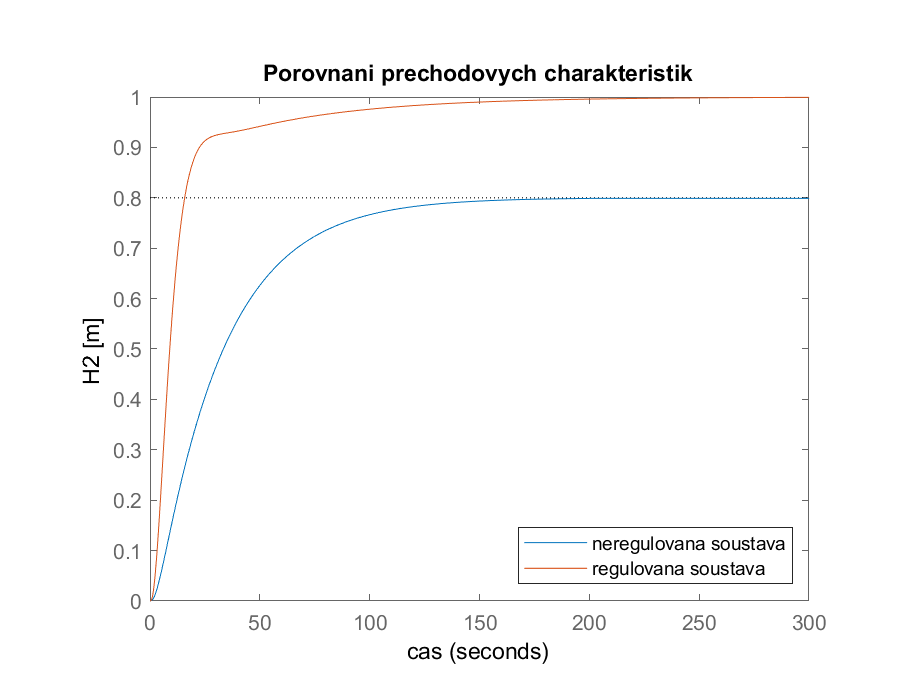
\includegraphics[width=0.7\textwidth]{./Graphics/graphs/C2/srovnani_reg_a_nereg_soustavy.eps}
				\caption{Odezva regulovaného a neregulovaného systému na jednotkový skok.}
				\label{pic:porovnani_regul_neregul_system}
			\end{figure}
			\begin{figure}[H]
				\centering
				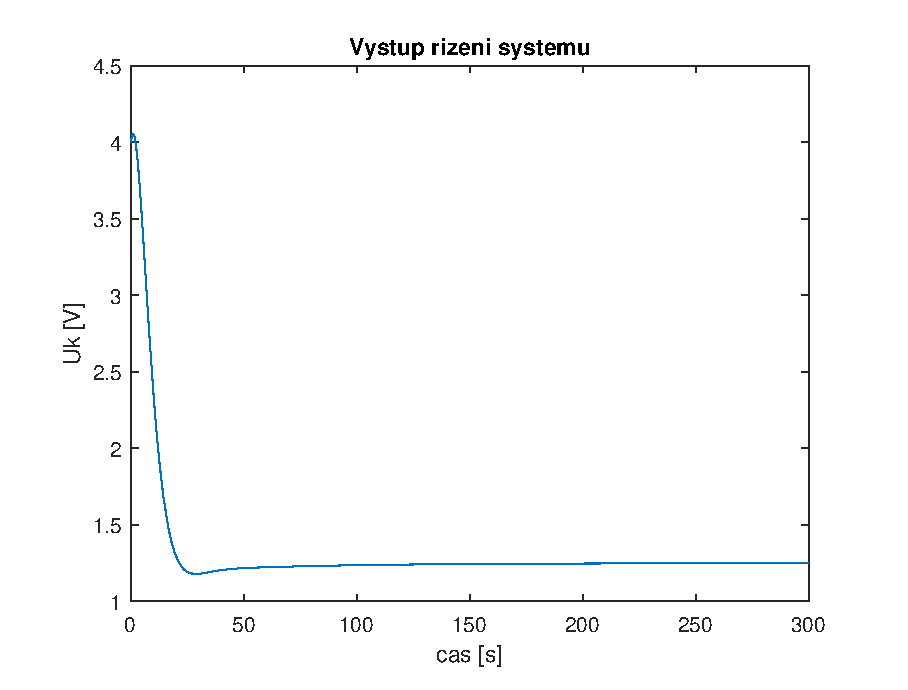
\includegraphics[width=0.7\textwidth]{./Graphics/graphs/C2/vystup_rizeni.eps}
				\caption{Výstupní signál regulátoru přiváděný na kotvu motoru čerpadla při odezvě na jednotkový skok (Obrázek \ref{pic:porovnani_regul_neregul_system}).}
				\label{pic:vystup_rizeni_regul_systemu}
			\end{figure}
			Nyní si stanovíme 4 různé body frekvenční charakteristiky (resp. harmonické frekvence) a dopočteme jejich polohu v komplexní rovině ze změřených hodnot odezvy systému.\\\\
			\textbf{Bod 1 }$\omega=0.01 rad/s$\\
			Perioda harm. vstupu: \(T_{in}=\frac{2\pi}{\omega}=\frac{2\pi}{0.01}=200\pi=628.3185\)\\
			Perioda výstupu: \(T_{out}=2\cdot(4385-4070)=630\)\\
			Fázový posun: \(\varphi=\frac{(3926-4070)}{T_{in}}=\frac{-144}{628.3185}=-0.229183 rad\rightarrow \varphi^{\circ}=-82.506^{\circ}\)\\
			Zesílení: \(K=\frac{13.24+0.4429}{2\cdot A_{in}}=\frac{13.6829}{2}=6.84145\)\hspace{1cm}\(A_{in}\dots\) amplituda vstupního signálu\\
			Souřadnice v komplexní rovině:\\
			\(B1_{Re}=K\cdot cos(\varphi)=6.84145\cdot cos(-82.506)=0.892278\)\\
			\(B1_{Im}=K\cdot sin(\varphi)=6.84145\cdot sin(-82.506)=-6.783014\)
			\begin{figure}[H]
				\centering
				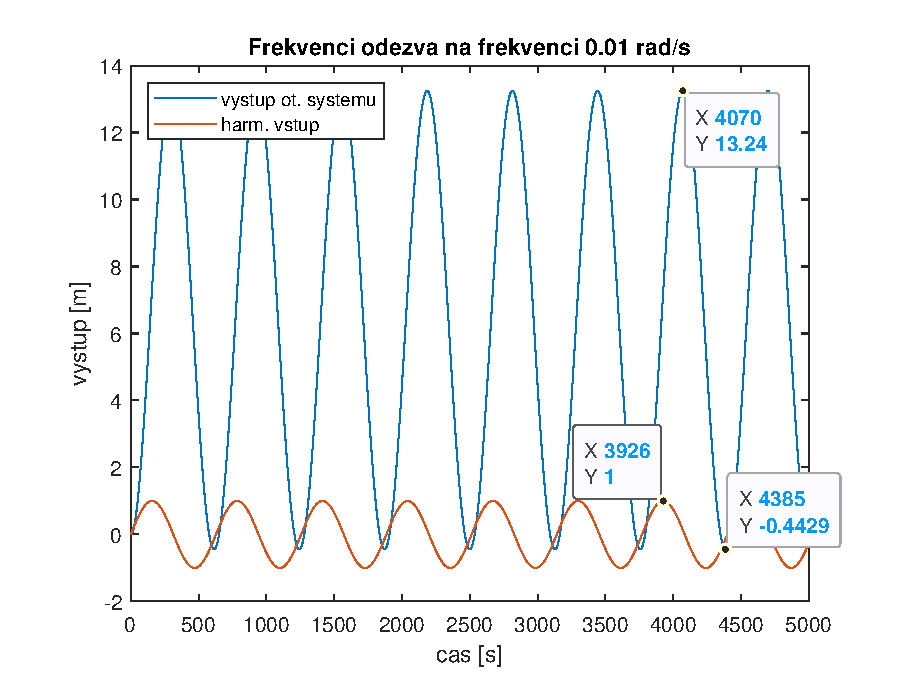
\includegraphics[width=.6\textwidth]{./Graphics/graphs/C2/odezva_harm_0.01.eps}
				\caption{Frekvenční odezva na harmonický signál o frekvenci \(0.01 rad/s\).}
				\label{pic:bod1}
			\end{figure}
			
			\noindent
			\textbf{Bod 2 }$\omega=0.05 rad/s$\\
			Perioda harm. vstupu: \(T_{in}=\frac{2\pi}{\omega}=\frac{2\pi}{0.05}=40\pi=125.6637\)\\
			Perioda výstupu: \(T_{out}=2\cdot(879.1-816.2)=125.8\)\\
			Fázový posun: \(\varphi=\frac{(785.1-816.2)}{T_{in}}=\frac{-31.1}{125.6637}=-0.247486 rad\rightarrow \varphi^{\circ}=-89.09496^{\circ}\)\\
			Zesílení: \(K=\frac{3.153+0.5934}{2\cdot A_{in}}=\frac{3.7464}{2}=1.8732\)\hspace{1cm}\(A_{in}\dots\) amplituda vstupního signálu\\
			Souřadnice v komplexní rovině:\\
			\(B1_{Re}=K\cdot cos(\varphi)=1.8732\cdot cos(-89.09496)=0.029588\)\\
			\(B1_{Im}=K\cdot sin(\varphi)=1.8732\cdot sin(-89.09496)=-1.872966\)
			\begin{figure}[H]
				\centering
				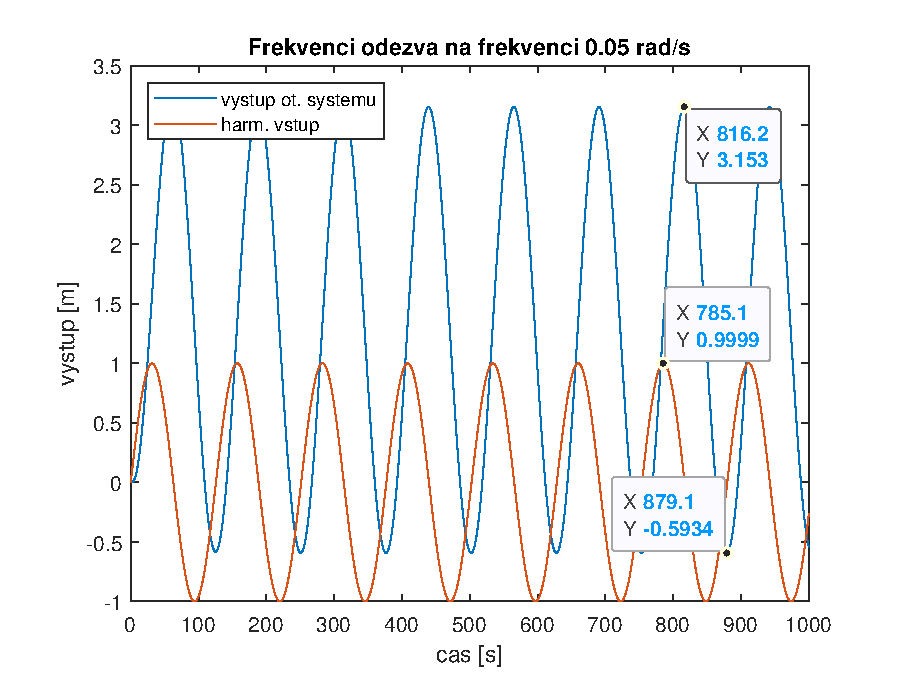
\includegraphics[width=.6\textwidth]{./Graphics/graphs/C2/odezva_harm_0.05.eps}
				\caption{Frekvenční odezva na harmonický signál o frekvenci \(0.05 rad/s\).}
				\label{pic:bod2}
			\end{figure}
			
			\noindent
			\textbf{Bod 3 }$\omega=0.1 rad/s$\\
			Perioda harm. vstupu: \(T_{in}=\frac{2\pi}{\omega}=\frac{2\pi}{0.1}=20\pi=62.8319\)\\
			Perioda výstupu: \(T_{out}=2\cdot(441.5-411.2)=60.6\)\\
			Fázový posun: \(\varphi=\frac{(393.1-411.2)}{T_{in}}=\frac{-18.1}{62.8319}=-0.288070 rad\rightarrow \varphi^{\circ}=-103.7052^{\circ}\)\\
			Zesílení: \(K=\frac{1.615+0.3364}{2\cdot A_{in}}=\frac{1.9514}{2}=0.9757\)\hspace{1cm}\(A_{in}\dots\) amplituda vstupního signálu\\
			Souřadnice v komplexní rovině:\\
			\(B1_{Re}=K\cdot cos(\varphi)=0.9757\cdot cos(-103.7052)=-0.231169\)\\
			\(B1_{Im}=K\cdot sin(\varphi)=0.9757\cdot sin(-103.7052)=-0.947920\)
			\begin{figure}[H]
				\centering
				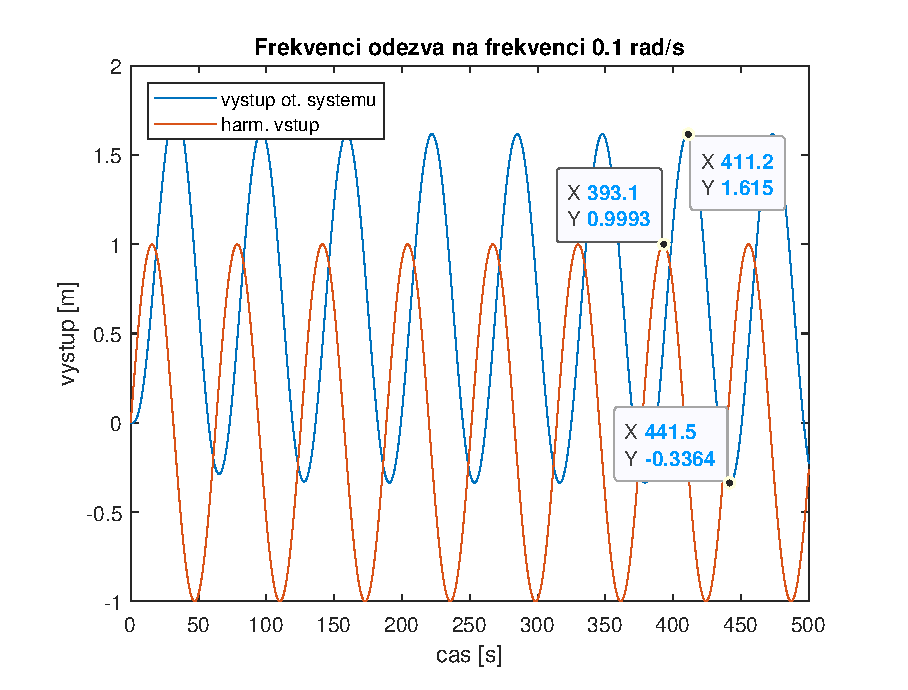
\includegraphics[width=.6\textwidth]{./Graphics/graphs/C2/odezva_harm_0.1.eps}
				\caption{Frekvenční odezva na harmonický signál o frekvenci \(0.1 rad/s\).}
				\label{pic:bod3}
			\end{figure}
			\noindent
			\textbf{Bod 4 }$\omega=0.5 rad/s$\\
			Perioda harm. vstupu: \(T_{in}=\frac{2\pi}{\omega}=\frac{2\pi}{0.5}=4\pi=12.566371\)\\
			Perioda výstupu: \(T_{out}=2\cdot(90.64-84.33)=12.62\)\\
			Fázový posun: \(\varphi=\frac{(78.68-84.33)}{T_{in}}=\frac{-5.65}{12.566371}=-0.449613 rad\rightarrow \varphi^{\circ}=-161.8607^{\circ}\)\\
			Zesílení: \(K=\frac{0.2479-0.01883}{2\cdot A_{in}}=\frac{0.22907}{2}=0.114535\)\hspace{1cm}\(A_{in}\dots\) amplituda vstupního signálu\\
			Souřadnice v komplexní rovině:\\
			\(B1_{Re}=K\cdot cos(\varphi)=0.114535\cdot cos(-161.8607)=-0.108843\)\\
			\(B1_{Im}=K\cdot sin(\varphi)=0.114535\cdot sin(-161.8607)=-0.035658\)
			\begin{figure}[H]
				\centering
				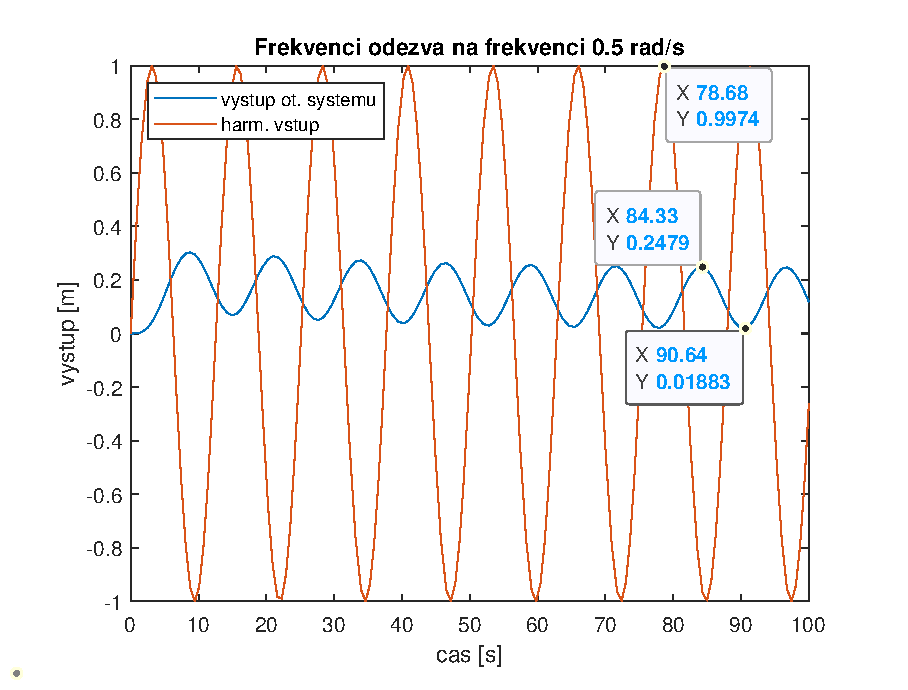
\includegraphics[width=.6\textwidth]{./Graphics/graphs/C2/odezva_harm_0.5.eps}
				\caption{Frekvenční odezva na harmonický signál o frekvenci \(0.5 rad/s\).}
				\label{pic:bod4}
			\end{figure}
			\noindent
			Necháme si vykreslit v Matlabu Nyquistovu křivku pomocí příkazu \verb*|nyquist(Fo)|, kde Fo je otevřený regulační obvod našeho systému. Do vykresleného grafu (Obrázek \ref{pic:nyquist}) si ještě zaneseme naše vypočtené čtyři body pomocí měření frekvenčních charakteristik. Odchylky ručně měřených bodů nemají takovou přesnost, přibližně ale potvrzují průběh Nyquistovy křivky našeho otevřeného regulačního obvodu.
			\begin{figure}[H]
				\centering
				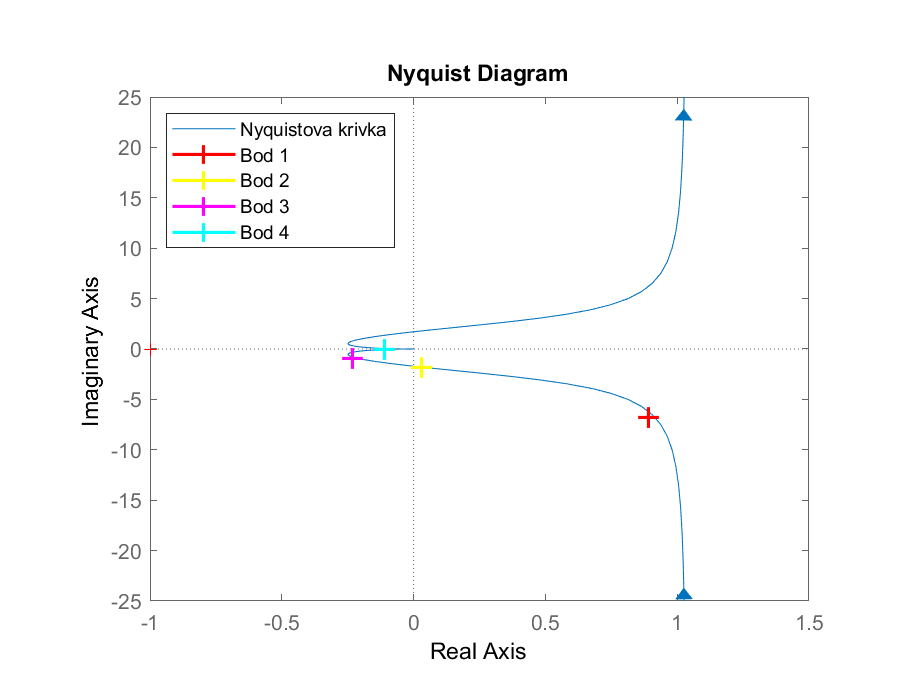
\includegraphics[width=.8\textwidth]{./Graphics/graphs/C2/nyquist.eps}
				\caption{Nyquistova křivka vykreslená pro otevřený regulační obvod včetně zakreslených 4 bodů ručně vypočtených}
				\label{pic:nyquist}
			\end{figure}
			\begin{figure}[H]
				\centering
				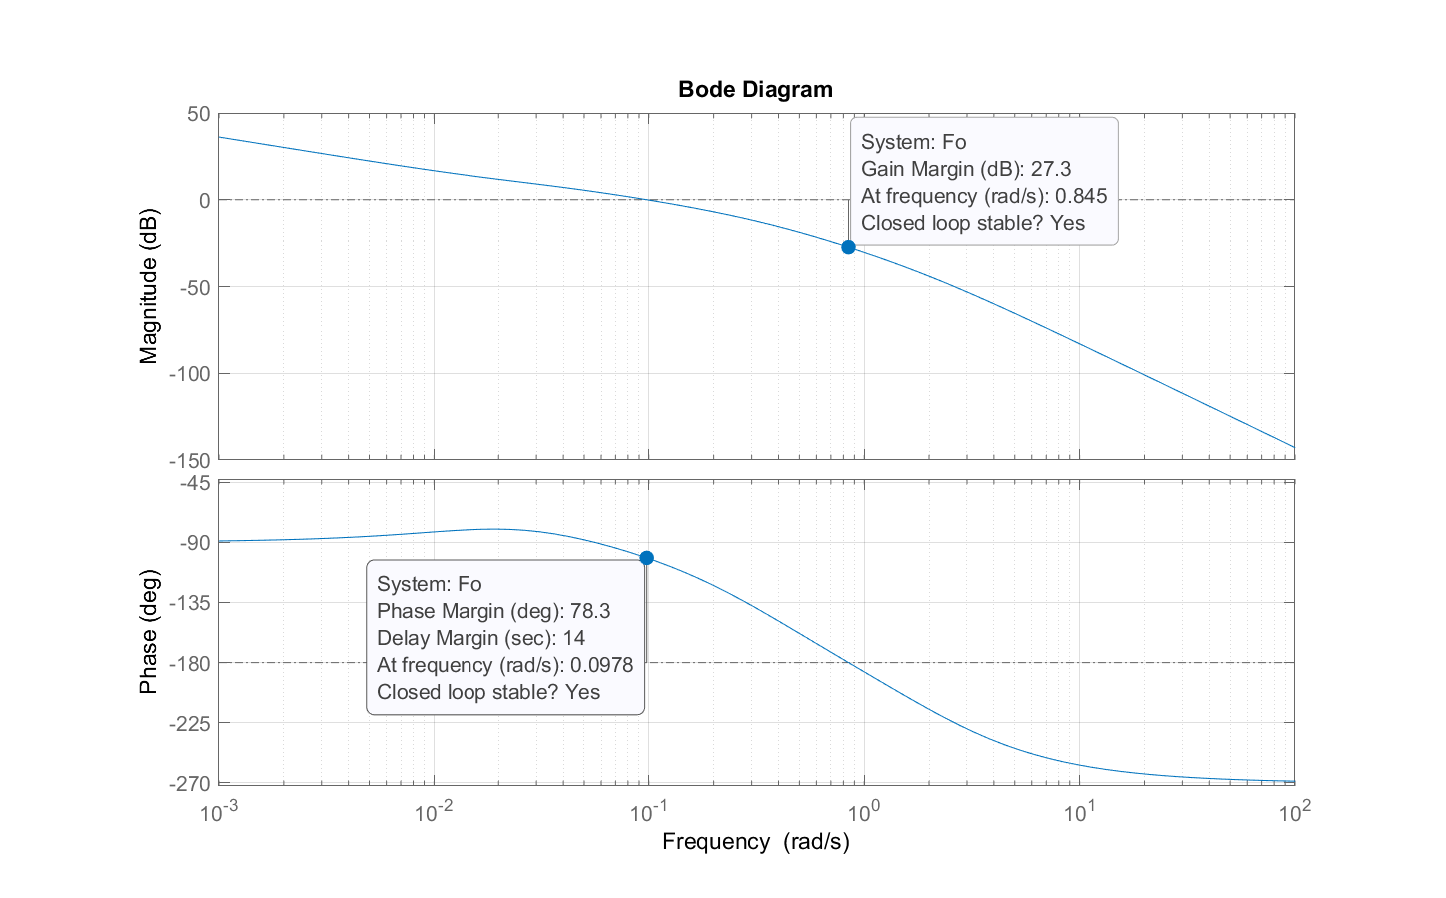
\includegraphics[width=\textwidth]{./Graphics/graphs/C2/bode.eps}
				\caption{Bodeho charakteristiky otevřeného regulačního obvodu.}
				\label{pic:bode}
			\end{figure}
			\noindent
			Z Bodeho charakteristik na obrázku \ref{pic:bode} můžeme přímo vyčíst bezpečnost v zesílení a ve fázi. Bezpečnost ve stabilitě určíme z citlivostní funkce ve tvaru
			\[S=\frac{1}{1+F_{o}}=\frac{50p^{4} + 118.8p^{3} + 38.06p^{2} + 1.125p}{50p^{4} + 118.8p^{3} + 38.06p^{2} + 4.725p + 0.072}.\]
			Po vykreslení Bodeho charakteristiky pro citlivostní funkci \(S\) můžeme zjistit její maximální zesílení přímo z obrázku \ref{pic:bode_S}.
			\begin{figure}[H]
				\centering
				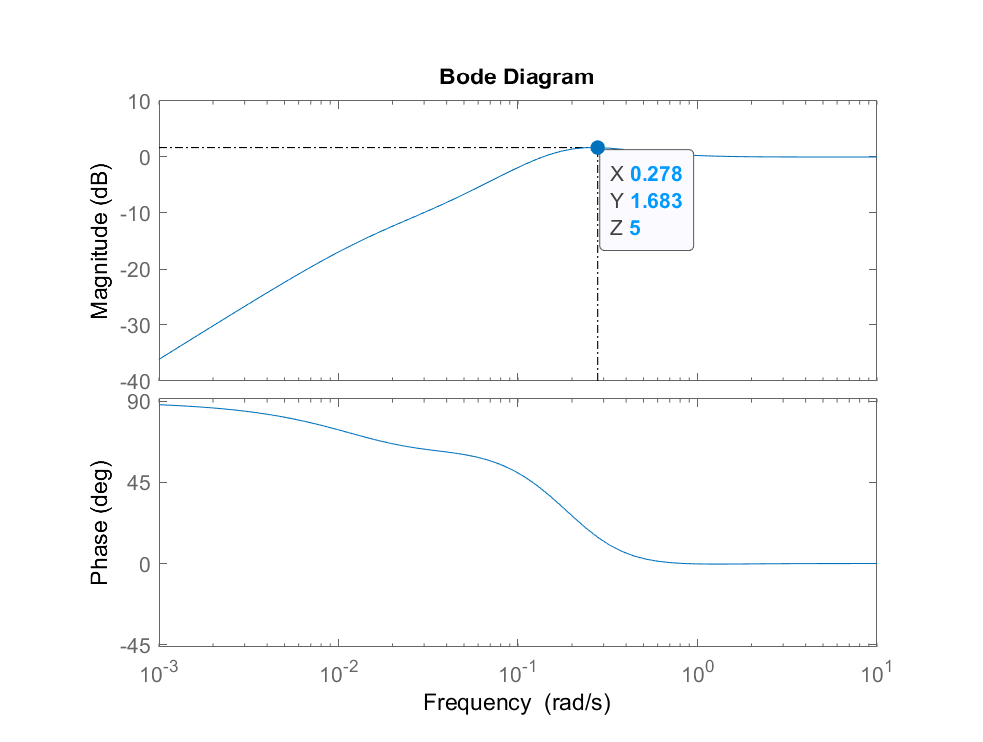
\includegraphics[width=\textwidth]{./Graphics/graphs/C2/bode_S.eps}
				\caption{Bodeho charakteristiky citlivostní funkce S.}
				\label{pic:bode_S}
			\end{figure}
			Maximální zesílení citlivostní funkce nám udává bezpečnost ve stabilitě odečtu tuto hodnotu z grafu na obrázku \ref{pic:bode_S}. Protože jsou charakteristiky v logaritmických souřadnicích, převedeme je.
			\[1.683=20\cdot log(S_{max})\]
			\[S_{max}=1.2138\]
			Pro zhodnocení práce regulátoru si vykreslíme přechodovou charakteristiku uzavřeného systému do obrázku \ref{pic:step_resp_Fu}.
			\begin{figure}[H]
				\centering
				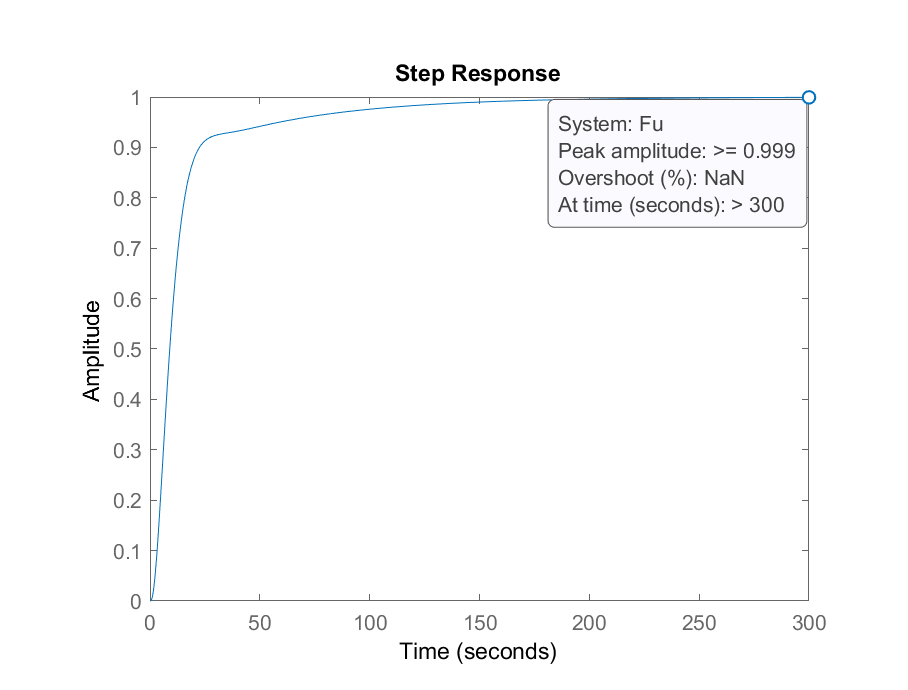
\includegraphics[width=.8\textwidth]{./Graphics/graphs/C2/step_resp_Fu.eps}
				\caption{Přechodová charakteristika uzavřeného systému.}
				\label{pic:step_resp_Fu}
			\end{figure}
			Přechodový děj probíhá velice pomalu a při snaze zvolit parametry regulátoru tak, aby nedošlo k překmitu došlo k tomu, že se systém ustálí až po delší době (\textgreater 300s). Je tedy velmi pomalý, ale po dostatečně dlouhé době se ustálí na požadované hodnotě.
		\subsection{Experimentální hledání kritického zesílení}
			Pomocí Hurwitzova kritéria stability zjistíme zesílení, při kterém dojde v uzavřeném obvodu k netlumenému kmitání. Hledáme kritické zesílení $K_{krit}$. To zjistíme pomocí charakteristické rovnice. Koeficienty dáme do Hurwitzovo matice a Hurwitzovo determinant $H_{n-1}$ se musí rovnat nule.
			\begin{center}
			charakteristická rovnice
			
			Za $T_i$ dosadíme 0,5. 
			
			\bigskip
			
			$0,5p^4+1,1875p^3+0,3806p^2+(0,01125+0,009K)p+0,018K=0$
			
			
			\bigskip
			
			Dosadíme koeficienty charakteristického polynomu
			
			\bigskip
			
			$\begin{bmatrix}
			1,1875 && 0,01125+0,009K && 0 && 0 \\
			0,5 && 0,3806 && 0,018K && 0 \\
			0 && 1,1875 && 0,01125+0,009K && 0 \\
			0 && 0,5 && 0,3806 && 0,018K
			\end{bmatrix}$
			
			\bigskip
			
			Teď vypočítáme Hurwitzovy determinanty.
			
			\bigskip
			
			$H_1=\begin{vmatrix}
			1,1875
			\end{vmatrix}=1,1875$
		
			\bigskip
			
			$H_2=\begin{vmatrix}
			1,1875 && 0,01125+0,009K\\
			0,5 && 0,3806 \\
			\end{vmatrix}=\frac{-360K+35707}{80000}$
		
			\bigskip
			
			$H_4=a_0H_3$
			
			\bigskip
			
			$H_3=\begin{vmatrix}
			1,1875 && 0,01125+0,009K && 0\\
			0,5 && 0,3806 && 0,018K\\
			0 && 1,1875 && 0,01125+0,009K \\
			\end{vmatrix}=\frac{-12960K^2-6853248K+1606815}{320000000}$
			
			\bigskip
			 Podmínka: $H_{n-1}=H_3=0$. Známe $H_3$ a z toho vypočítáme zesílení $K$, když determinant položíme rovno nule.
			 
			 \bigskip
			 
			 $\frac{-12960K^2-6853248K+1606815}{320000000}=0$
			 
			 \bigskip
			 
			 Podmínka pro zesílení je $K > 0$.
			 
			 \bigskip
			 
			 $K=K_{krit}=0,234356497581$
			\end{center}
				\begin{figure}[H]
					\centering
					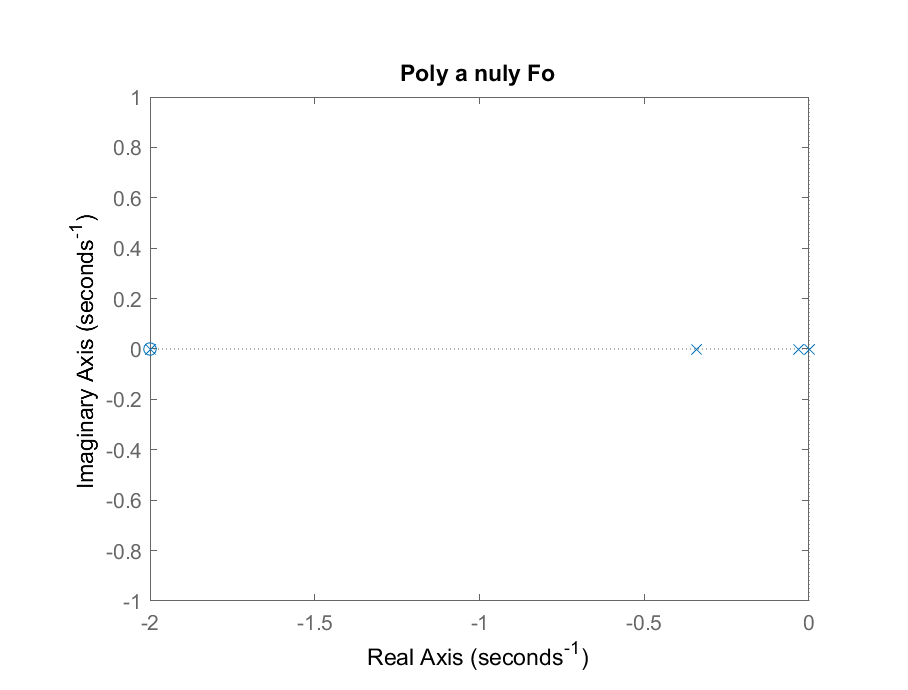
\includegraphics[width=.6\textwidth]{./Graphics/graphs/D2/poly_nuly_Fo.eps}
					\caption{Nuly a póly otevřené smyčky.}
				\end{figure}
				\begin{figure}[H]
					\centering
					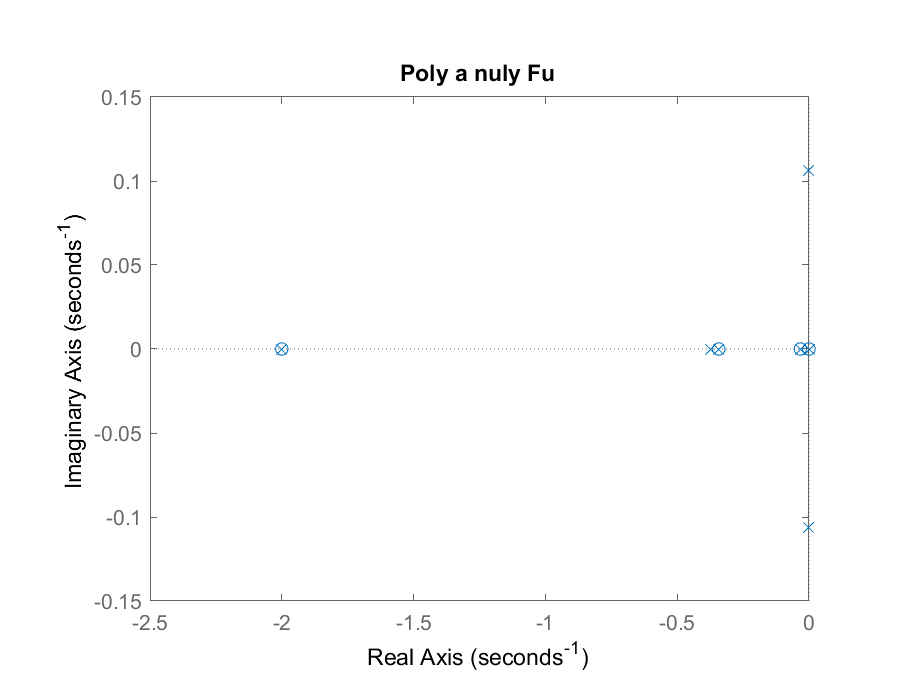
\includegraphics[width=.6\textwidth]{./Graphics/graphs/D2/poly_nuly_Fu.eps}
					\caption{Nuly a póly uzavřené smyčky.}
				\end{figure}
				\begin{figure}[H]
					\centering
					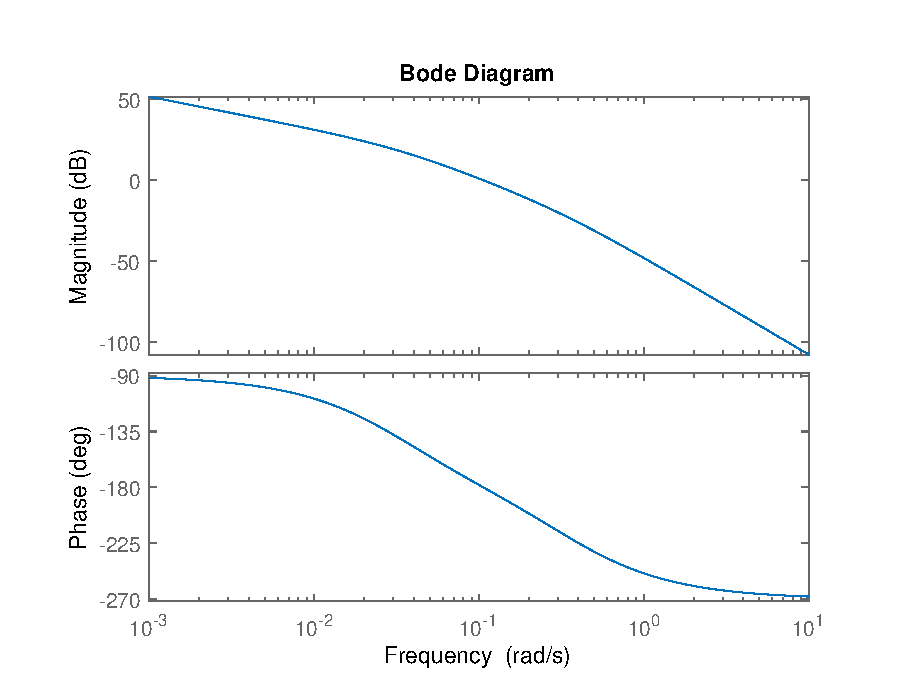
\includegraphics[width=.6\textwidth]{./Graphics/graphs/D2/bode_Fo.eps}
					\caption{Bodeho charakteristika otevřené smyčky.}
				\end{figure}
				\begin{figure}[H]
					\centering
					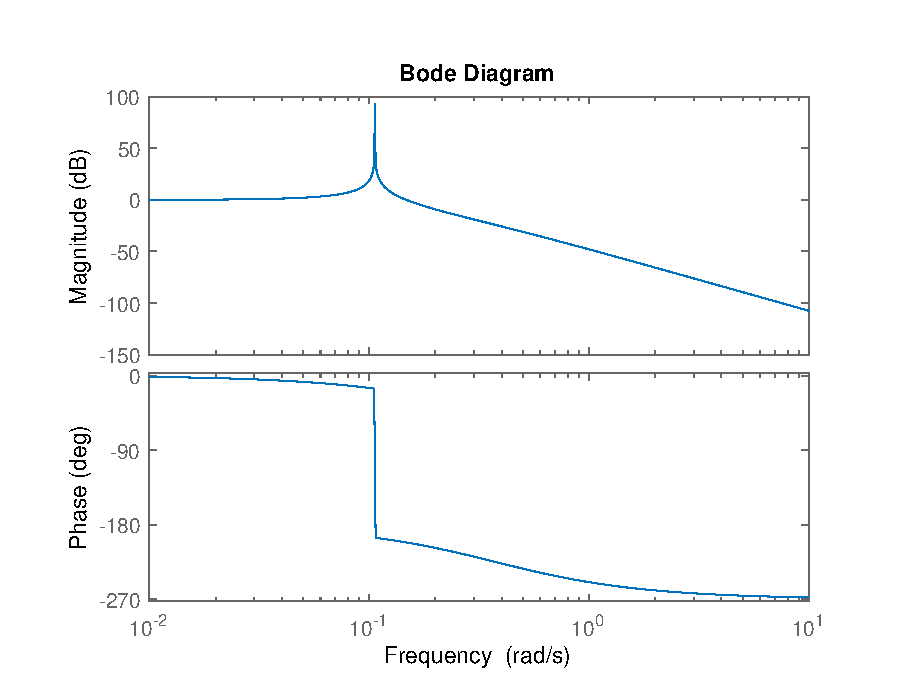
\includegraphics[width=.6\textwidth]{./Graphics/graphs/D2/bode_Fu.eps}
					\caption{Bodeho charakteristika uzavřené smyčky.}
				\end{figure}
				\begin{figure}[H]
					\centering
					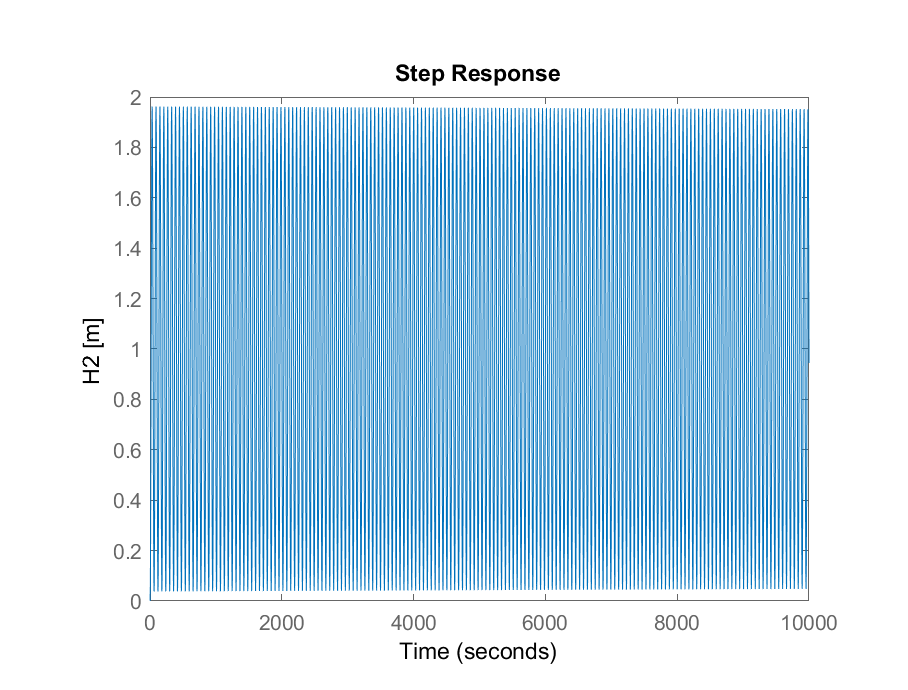
\includegraphics[width=.6\textwidth]{./Graphics/graphs/D2/odezva_skok_K_krit_short}
					\caption{Přechodová charakteristika pro systém s nastaveným zesílením \(K=K_{krit}\) pro omezenou délku trvání simulace.}
					\label{pic:D2_krit_zes1}
				\end{figure}
				\begin{figure}[H]
					\centering
					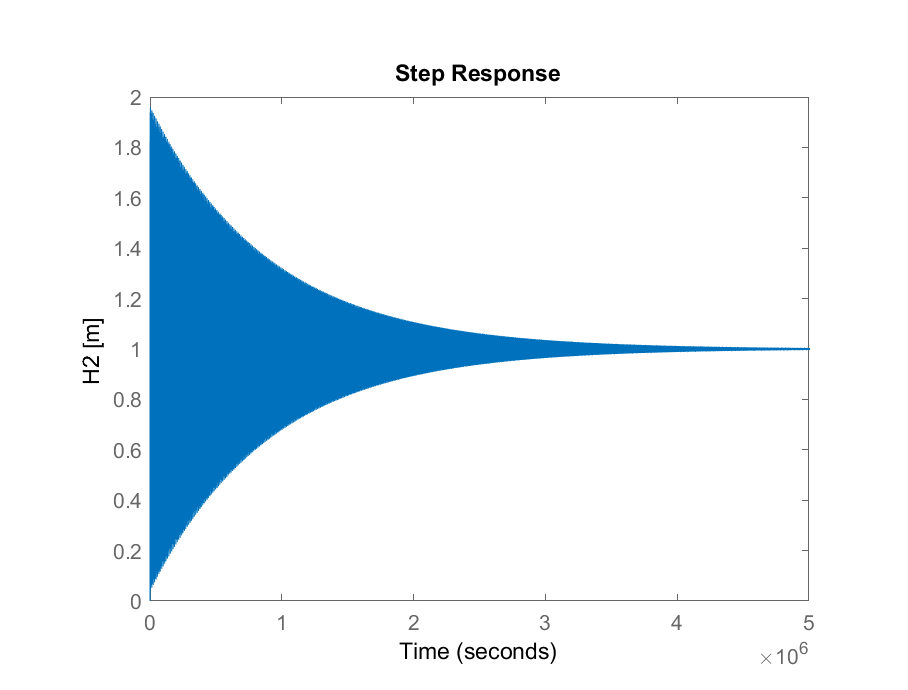
\includegraphics[width=.6\textwidth]{./Graphics/graphs/D2/odezva_skok_K_krit_long}
					\caption{Přechodová charakteristika pro systém s nastaveným zesílením \(K=K_{krit}\).}
					\label{pic:D2_krit_zes2}
				\end{figure}
				V obrázcích \ref{pic:D2_krit_zes1} a \ref{pic:D2_krit_zes2} lze vidět, že při kritickém zesílením dochází ke kmitání výstupu, ale z druhého obrázku je patrné, že se po delší době ustálí. To může být způsobeno chybou ve výpočtu nebo zaokrouhlením.
		\subsection{Odvození parametrů PI regulátoru}
			V tomto bodě budeme odvozovat pomocí GMK parametry PI regulátoru. Opět budeme pracovat s přenosem uzavřené smyčky. 
			\[F=\frac{0,018K(T_ip+1)}{T_ip(p^3 + 2,375 p^2 + 0,7612 p + 0,0225)+(T_ip+1)0,018K}\]
			
			Rozložíme čitatele i jmenovatel na součin.
			\[F=\frac{0,018KT_i(p+\frac{1}{T_i})}{T_ip(p^3 + 2,375 p^2 + 0,7612 p + 0,0225)+(T_ip+1)0,018K}\]
			Pro tento přenos zvolíme vhodné umístění pólů, ze kterých vypočítáme parametry PI regulátoru. Systém má jednu nulu, $m=1$, $z_1=-\frac{1}{T_i}$, a čtyři póly, $n=4$, $p_1=-2,0015$, $p_2=-0,3721$, $p_3= -0,0007 + 0,1149i$, $p_4= -0,0007 - 0,1149i$. GMK má tři asymptoty. Pro tento přenos odpovídají parametry regulátoru těmto hodnotám $\rightarrow$ $T_i=0,86$ a $K=0,47$. Z toho plyne, že nula $z_1=-\frac{50}{43}$. Systém vypadá takto 
			\[F=\frac{0,0072756(p+\frac{50}{43})}{(p+2,0015)(p+0,3721)(p+0,0007 + 0,1149i)(p+0,0007 - 0,1149i)}.\]
			
			Jelikož je splněna podmínka $n-m \geq 2$, znamená to, že součet pólů otevřené smyčky se rovná součtu pólů uzavřené smyčky.
			
			\begin{center}
			Vypočítáme bod, kde se potkávají všechny asymptoty.
			
			\bigskip
			
			$q=\frac{\sum_i p_i - \sum_j z_j}{n-m}=\frac{-2,0015-0,3721-0,0007+0,1149i-0,0007-0,1149i+\frac{50}{43}}{3}=- 0,6667$
			
			\bigskip
			
			Teď vypočítáme asymptoty, které jsou tři. $l=1$, $2$, $3$.
			
			\bigskip
			
			$\alpha_l=\frac{\pi+(l-1)2\pi}{n-m}$
			
			$\alpha_1=\frac{\pi}{3}=60^{\circ}$
			
			$\alpha_2=\frac{\pi+2\pi}{3}=\pi=180^{\circ}$
			
			$\alpha_3=\frac{\pi+4\pi}{3}=\frac{5\pi}{3}=300^{\circ}$
			
			\bigskip
			
			Nakonec vypočítáme body, kdy větve přechází na reálnou osu.
			
			\bigskip
			
			$\sum_i \frac{1}{p-p_i}-\sum_j \frac{1}{p-z_j}=0$
			
			$\frac{1}{p+2,0015}+\frac{1}{p+0,3721}+\frac{1}{p+0,0007-0,114i}+\frac{1}{0,0007+0,1149i}-\frac{1}{p+\frac{50}{43}}=0$
			
			\bigskip
			
			Vyjdou nám 4 kořeny. 
			
			\bigskip
			
			$p_1=-0,017197222107058621890968543792558$
			
			$p_2=-0,23639720257288979616816068858502$
			
			$p_3=- 1.4400632527763048607378772442763 - 0.45514565317143789661943736324585i$
			
			$p_4=- 1.4400632527763048607378772442763 + 0.45514565317143789661943736324585i$
			
			\bigskip
			
			
			\end{center}
			
			\bigskip
			
Systém neprotíná imaginární osu, a tudíž nemá žádné kritické zesílení.
			
			Vytvoříme přenos systému pro otevřenou smyčku, který má tvar $F(p)=F_R(p)F_S(p)$.
			\begin{center}
			$F(p)=F_R(p)F_S(p)=K(1+\frac{1}{T_ip})\frac{0,018}{p^3 + 2,375 p^2 + 0,7612 p + 0,0225}=\frac{0,018KT_ip+0,018K}{T_ip(p^3 + 2,375 p^2 + 0,7612 p + 0,0225)}=\frac{0,018KT_i(p+\frac{1}{T_i})}{T_ip(p+0,0328862422062)(p+2,00003066251)(p+0,342083095279)}$
			\end{center}
			
			Tento systém má $m=1$ nul, $z_1=-\frac{1}{T_i}$ jako uzavřený systém a počet pólů je taky stejný, jak už jsme uvedli výše. $n=4$, $p_1=0$,  $p_2=-0,0328862422062$, $p_3=-2,00003066251$, $p_4=-0,342083095279$. 
			
			Dosadíme výše zmíněné zesílení $K=0,47$ a časovou konstantu $T_i=0,86$. Vyjde nám, že nula systému je opět $z_1=-\frac{50}{43}$.
			
			Regulátor z předchozího příkladu měl kritické zesílení $K_{krit}=0,234356497581$ a regulátor vypočítaný v tomto úkolu žádné kritické zesílení nemá. 
				\begin{figure}[H]
					\centering
					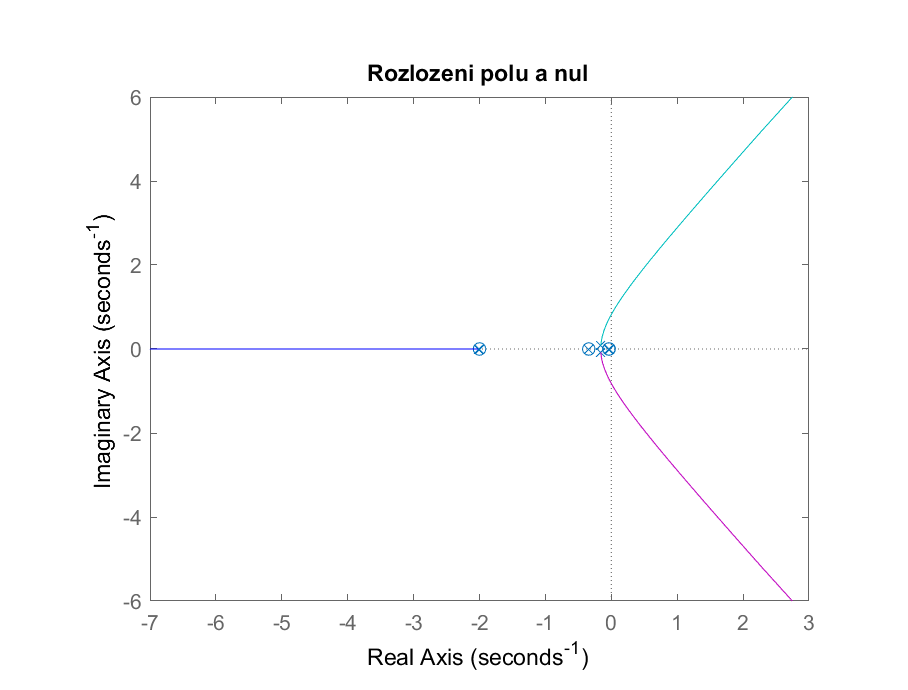
\includegraphics[width=.8\textwidth]{./Graphics/graphs/E2/rlocus}
					\caption{GMK s dodatečně přidaným pólem v bodě \([0; 0j]\) a nulou nastavenou podle zakřivení křivek.}
				\end{figure}
				\begin{figure}[H]
					\centering
					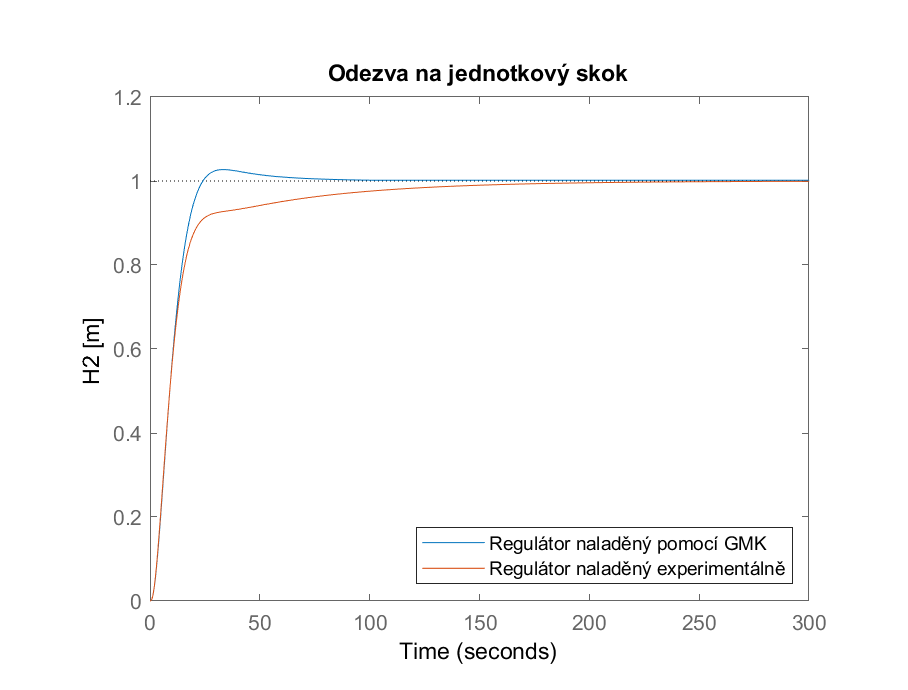
\includegraphics[width=.8\textwidth]{./Graphics/graphs/E2/sorvnani_regulatoru}
					\caption{Porovnání systémů s regulátorem nastaveným experimentálně a pomocí GMK.}
				\end{figure}
		\subsection{Dopravní zpoždění}
				\begin{figure}[H]
					\centering
					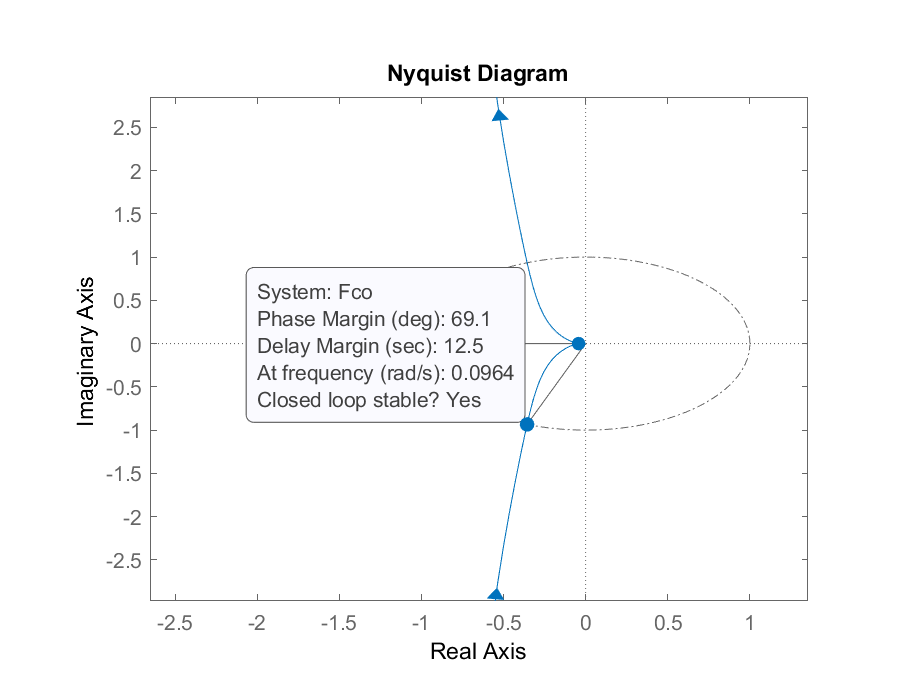
\includegraphics[width=.8\textwidth]{./Graphics/graphs/E2/nyquist_Fco}
					\caption{Nyquistova charakteristika otevřeného regulačního obvodu, z které je patrné mezní dopravní zpoždění.}
				\end{figure}
				\begin{figure}[H]
					\centering
					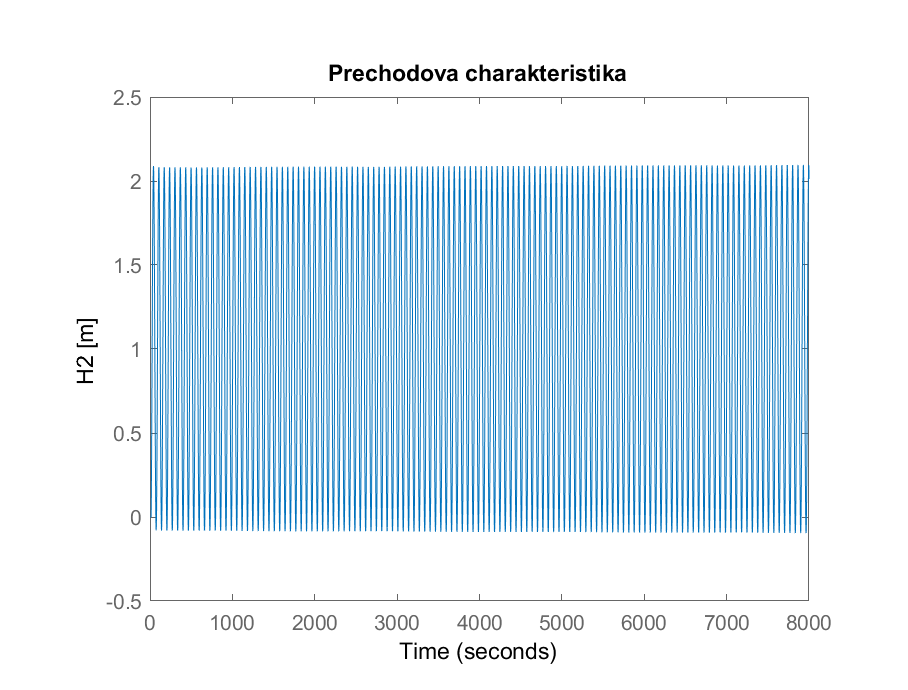
\includegraphics[width=.8\textwidth]{./Graphics/graphs/F2/Prechodova_charakteristika_zpozdeni_12.518}
					\caption{Přechodová charakteristika systému s regulátorem naladěným podle GMK s dopravním zpožděním \(D=12.518\)}
				\end{figure}
			Posledním úkolem je uvažovat, že řízený systém má dopravní zpoždění. V příkladu výše jsme pracovali se zesílením $K=0,47$ a časovou konstantu $T_i=0,86$. Máme určit takové dopravní zpoždění, aby se náš systém dostal na mez asymptotické stability. Přenos dopravního zpoždění je
			\[F=e^{-Dp}.\]
			
			Ze systému 
			\[F=\frac{0,0072756(p+\frac{50}{43})}{(p+2,0015)(p+0,3721)(p+0,0007 + 0,1149i)(p+0,0007 - 0,1149i)}\]
			 vytvoříme uzavřenou smyčku s dopravním zpožděním. Výsledný systém bude vypadat 
			\begin{center}
			$F=\frac{\frac{0,0072756(p+\frac{50}{43})}{(p+2,0015)(p+0,3721)(p+0,0007 + 0,1149i)(p+0,0007 - 0,1149i)} e^{-Dp}}{1+\frac{0,0072756(p+\frac{50}{43})}{(p+2,0015)(p+0,3721)(p+0,0007 + 0,1149i)(p+0,0007 - 0,1149i)e^{Dp}} }=\frac{0,0072756(p+\frac{50}{43})}{(p+2,0015)(p+0,3721)(p+0,0007 + 0,1149i)(p+0,0007 - 0,1149i) e^{Dp}+0,0072756(p+\frac{50}{43})}$
			\end{center}
		$D$ bude dopravní zpoždění.
		
			 Systém bude na mezi asymptotické stability, pokud se reálné části pólů budou rovnat nule.
			  \begin{center}
			  charakteristický polynom
			  
			  \bigskip
			  
			  $(p+2,0015)(p+0,3721)(p+0,0007 + 0,1149i)(p+0,0007 - 0,1149i) e^{Dp}+0,0072756(p+\frac{50}{43})=0$
			  \end{center}
			  
			  Náš systém se nikdy nemůže dostat na mez asymptotické stability, jelikož pro $p=0$ nezáleží na dopravním zpoždění $D$.
\end{document}
